\documentclass[review]{siamart220329}

\usepackage{url}
\usepackage[hmargin=1.5in]{geometry}
\usepackage{enumitem}
\usepackage{amsmath}
\usepackage{amssymb}
%%\usepackage{amsthm}
\usepackage{graphicx}
%%\usepackage[svgnames]{xcolor} % for verifications
\usepackage{environ} % to hide verifications
\usepackage{tikz}

% TikZ libraries
\usetikzlibrary{bbox}
\usetikzlibrary{fadings}
\usetikzlibrary{cd}

% hat tip TeX.SE user Andrew Stacey
%   https://tex.stackexchange.com/a/82503/6934
%   https://tex.stackexchange.com/questions/82425/tikz-radial-shading-of-a-ring#comment176908_82503
\pgfdeclareradialshading{radialedge}{\pgfpointorigin}{%
  color(0bp)=(transparent!0);
  color(20bp)=(transparent!0);
  color(22bp)=(transparent!10);
  color(24bp)=(transparent!90);
  color(25bp)=(transparent!100)
}
\pgfdeclarefading{radial edge}{\pgfuseshading{radialedge}}%

\setcounter{tocdepth}{2}

\newsiamremark{rmk}{Remark}

% list formatting
\newlist{conditions}{itemize}{1}
\setlist[conditions]{leftmargin=26mm, rightmargin=12mm}
\makeatletter
% hat tip TeX.SE user31729
%   https://tex.stackexchange.com/a/328393/6934
\newcommand{\cond}[1]{\item[(\textsc{#1})]\protected@edef\@currentlabel{\textsc{#1}}}
\newcommand{\condconst}[2]{\item[($\text{\textsc{#1}} \mid #2$)]\protected@edef\@currentlabel{$\text{\textsc{#1}} \mid #2$}}
\makeatother

% convenience aliases
\newcommand{\maps}{\colon}

% group action
\newcommand{\acts}{\mathbin{\raisebox{\depth}{\rotatebox{-90}{$\circlearrowright$}}}}

% symbology
\newcommand{\N}{\mathbb{N}}
\newcommand{\Z}{\mathbb{Z}}
\newcommand{\R}{\mathbb{R}}
\newcommand{\C}{\mathbb{C}}
\let\Re\relax
\DeclareMathOperator{\Re}{Re}
\newcommand{\laplace}{\mathcal{L}}
\newcommand{\series}[1]{\tilde{#1}}
\newcommand{\fracderiv}[3]{\partial^{#1}_{#2, #3}}

% function spaces
\newcommand{\cont}{\mathcal{C}}
\newcommand{\holo}{\mathcal{H}}
\newcommand{\singexp}[2]{\mathcal{H}L^\infty_{#1, #2}}
\newcommand{\singexpalg}[1]{\singexp{#1}{\bullet}}
\newcommand{\holoL}[1]{\mathcal{H}L^{#1}} %% may no longer be needed
\newcommand{\expHoloL}[2]{\mathcal{H}L^{#1}_{#2}} %% may no longer be needed

% operator under consideration
\newcommand{\genvolterra}{\mathcal{W}}
\newcommand{\genker}{w}
\newcommand{\volterra}{\mathcal{V}}
\newcommand{\hardpart}{\mathcal{V}_0}
\newcommand{\softpart}{\mathcal{V}_\star}
\newcommand{\kerwhole}{k}
\newcommand{\hardker}{k_0}
\newcommand{\softker}{k_\star}
\newcommand{\solwhole}{f}
\newcommand{\solproto}{f_0}
\newcommand{\solptb}{f_\star}
\newcommand{\roots}{\mathfrak{B}}

% domain
\newcommand{\domain}{\Omega}
\newcommand{\near}{\Omega_\text{near}}
\newcommand{\far}{\Omega_\text{far}}

% drafting environments
\newenvironment{brainstorm}{\color{violet}\begin{itemize}}{\end{itemize}\color{black}}

% hideable verifications
\newif\ifshowverify
\showverifyfalse
\ifshowverify
\newenvironment{verify}{\color{veriforest}}{\color{black}}
\else
\NewEnviron{verify}{\iffalse\expandafter\BODY\fi}
\fi

% colors
\definecolor{ietocean}{RGB}{0, 30, 140}
\definecolor{ietcoast}{RGB}{0, 150, 173}
\definecolor{ietlagoon}{RGB}{0, 216, 180}
\definecolor{veriforest}{RGB}{0, 80, 40}

% pretty prince hyperref must always be the last thing in the preamble, always
\usepackage{hyperref}
\hypersetup{
  colorlinks,
  linkcolor={ietcoast},
  citecolor={ietcoast},
  urlcolor={ietcoast}
}

\title{Regular singular Volterra equations on complex domains}
\author{Veronica Fantini and Aaron Fenyes}
\date{}

\begin{document}
\maketitle

\begin{abstract}
The inverse Laplace transform can turn a linear differential equation on a complex domain into an equivalent Volterra integral equation on a real domain. This can make things simpler: for example, a differential equation with irregular singularities can become a Volterra equation with regular singularities. It can also reveal hidden structure, especially when the Volterra equation extends to a complex domain. Our main result is to show that for a certain kind of regular singular Volterra equation on a complex domain, there is always a unique solution of a certain form. As a motivating example, this kind of Volterra equation arises when using Laplace transform methods to solve a {\em level~1} differential equation.
\end{abstract}
\tableofcontents
\section{Introduction}\label{sec:intro}
\subsection{Motivation}\label{motivation}
\color{blue}
\textcolor{blue}{An ordinary differential equation with an irregular singularity at infinity comes with a special family of formal solutions: ``normal series'' characterized by their formal asymptotics at infinity~\cite{int-irreg}. These series are typicaly divergent, but they can be ``resummed'' to produce analytic solutions~\cite{loday1994stokes,diverg-resurg--ii,loday-Remy2011,malgrange1995sommation,ramis1991series}. The results of this paper are motivated by the desire to find the same analytic solutions more directly, without the use of formal series. We do this in Section~\ref{sec:example} for a certain class of level~$1$ ODEs, using new Laplace transform methods tailored to the special properties of the analytic solutions that we seek. In~\cite{borel_reg}, we show that these solutions match the ones obtained through resummation. Since the Laplace transform methods we use may be of wider interest, we describe them here in a general and self-contained way.}

In its most basic form, the Laplace transform $\laplace$ turns exponential-type functions of a real ``position'' variable $\zeta$ into holomorphic functions of a complex ``frequency'' variable $z$. \begin{verify}[Suppose the magnitude of the Laplace transform integrand is Riemann-integrable on $(0, \infty)$. Write $z$ in terms of its real and imaginary parts as $x + iy$. Since the integrand is holomorphic with respect to $z$, the operator $\frac{\partial}{\partial\overline{z}} = \frac{1}{2}\left(\frac{\partial}{\partial x} + i\frac{\partial}{\partial x}\right)$ annihilates it. Using the comparison version of Leibniz's rule for improper integrals (Theorem~11.10 of A First Course in Real Analysis, by Protter and Morrey) with $\frac{\partial}{\partial x}$ and $\frac{\partial}{\partial y}$, we see that $\frac{\partial}{\partial\overline{z}}$ annihilates the whole integral.]\end{verify} Through identities like
\begin{align*}
\frac{\partial}{\partial z} \laplace \varphi & = \laplace(-\zeta\varphi) \\
\laplace k\;\laplace \varphi & = \laplace(k * \varphi) \\
z^{-\nu} \laplace \varphi & = \laplace\,\partial^{-\nu} \varphi,
\end{align*}
where $\partial^{-\nu}$ is the Riemann-Liouville fractional integral of order $\nu \in (0, \infty)$, the Laplace transform pulls differential operators on the frequency domain back to Volterra integral operators on the position domain. The favorable regularity properties and comprehensive theory of Volterra equations can thus be brought to bear on linear differential equations.

Some differential equations pull back to Volterra equations with real-analytic kernels, which extend to holomorphic Volterra equations on complex extensions of the position domain. For instance, in Section~\ref{sec:example}, we consider equations of the form
\begin{equation}\label{eqn:intro-level-1}
\left[ P\big(\tfrac{\partial}{\partial z}\big) + \frac{1}{z} Q\big(\tfrac{\partial}{\partial z}\big) + \frac{1}{z^2} R(z^{-1}) \right] \Phi = 0
\end{equation}
given by polynomials $P$, $Q$ and a holomorphic function $R(z^{-1})$ satisfying some extra conditions. A function of the form $\Phi = \laplace \varphi$ satisfies this equation if and only if $\varphi$ satisfies the integral equation
\begin{equation}\label{eqn:intro-use-dict}
\big[ P(-\zeta)+\partial^{-1}\circ Q(-\zeta)+\partial^{-2}\circ R(\partial^{-1}) \big] \varphi = 0.
\end{equation}
The integral operator remains well-defined if we make $\zeta$ a complex coordinate and seek solutions $\varphi$ which extend holomorphically into the complex position domain.

Equation~\eqref{eqn:intro-level-1} can be solved by resumming normal series, as described earlier. Each resummed solution is characterized by its $e^{-\alpha z} z^{-\tau_\alpha}$ asymptotics, where $-\alpha$ is a root of $P$ and $\tau_\alpha = Q(-\alpha)/P'(-\alpha)$ is real and positive. To obtain this solution analytically through Laplace transform methods, we must take the Laplace transform $\laplace_{\zeta,\alpha}$ that uses $\zeta = \alpha$ in place of the traditional $\zeta = 0$ as the integration base point. Equation~\eqref{eqn:intro-use-dict} then comes out based at $\zeta = \alpha$ as well. We seek a solution $\psi_\alpha$ which
\begin{itemize}
\item has an $O\big((\zeta - \alpha)^{\tau_\alpha-1}\big)$ singularity at $\zeta = \alpha$; and
\item is of exponential type, meaning that it is $O\big(e^{\Lambda|\zeta|}\big)$ for some $\Lambda \in \R$ as $\zeta$ grows.
\end{itemize}
These conditions ensure that $\psi_\alpha$ has a well-defined Laplace transform, and the first condition gives $\laplace_{\zeta, \alpha} \psi_\alpha$ the desired asymptotics.

The theory of Volterra equations is well-suited to this solution method. By embodying our conditions on $\psi_\alpha$ in a Banach space, defined in Section~\ref{fn-spaces}, we can solve equations like~\eqref{eqn:intro-use-dict} using the contraction mapping theorem, taking advantage of the regularizing effect of the relevant Volterra operators. This establishes the existence and uniqueness of $\psi_\alpha$, as stated in Theorem~\ref{thm:example}. Since integral operators on the position domain correspond directly to multiplication operators on the frequency domain, with no need to worry about initial values, we know immediately that $\laplace_{\zeta, \alpha} \psi_\alpha$ satisfies equation~\eqref{eqn:intro-level-1}, even when $\psi_\alpha$ blows up at $\zeta = \alpha$. By isolating the features of equation~\eqref{eqn:intro-use-dict} that make our contraction mapping argument possible, we get the main result of this paper: the general existence and uniqueness result stated in Section~\ref{sec:results}.

Our results build on known methods for solving differential equations with irregular singularities. Our focus on integral equations in the position domain, and the singularities of their solutions, \textcolor{orange}{recalls [reword]} \'{E}calle's \textcolor{orange}{[and Remy \& Loday-Richaud's?]} theory of resurgence~\cite{EcalleIII}. One of our motivations is to understand \'{E}calle's theory from an analytic perspective, without reference to formal solutions. The Banach spaces we use to achieve this also appear in the work of Braaksma, who uses them to solve systems of ODEs whose coefficients are expressed as Laplace transforms~\cite{braaksma2006laplace}. This overlap suggests an opportunity to combine the two approaches, extending our results to systems of equations, and Braaksma's to equations with more general coefficients.
\subsection{Formalism for coordinates}
Our motivating example, equation~\eqref{eqn:intro-use-dict}, has regular singularities at various points $\zeta = \alpha$ on the position domain. Each associated solution $\psi_\alpha$ is most easily expressed in terms of its own translated position coordinate $\zeta_\alpha = \zeta - \alpha$. We therefore expect our results to be used in calculations involving multiple coordinates. Our formalism for points, functions, and coordinates is tailored to such calculations.

From now on, we will carefully respect the distinction between points and coordinates. A point is a location in space, while a coordinate is a function on space. For example, the position coordinates $\zeta$ and $\zeta_\alpha$ are functions on the position domain, just like the integral equation solutions $\psi_\alpha$. A coordinate, like $\zeta$, can be evaluated at a point $b$, yielding a number $\beta := \zeta(b)$. Conversely, the point $b$ can be described as the place where $\zeta = \beta$.

\textcolor{orange}{[talk about integration]} For a function $\varphi$ defined on a simply connected subset of the position domain,

%%Coordinates, like the frequency coordinate $z$ and the position coordinates $\zeta$ and $\zeta_\alpha$,

%%We will typically speak in terms of functions on spaces, not functions of coordinates.

%%Functions---like the coordinates $\zeta$ and $\zeta_\alpha$, and the solutions $\psi_\alpha$---will be defined directly on the position or frequency domain, not as functions of a particular coordinate.

\textcolor{orange}{[\ldots]}
\color{violet}
\begin{itemize}
\item Can mention translation surfaces, but don't define.
\item Maybe talk about branched covers of the complex plane, which we need to describe the singular solutions?
\item Can identify the number $\zeta(a)$ with the point $a$.
%%\item In the theory of resurgence, the position domain is often a Riemann surface $B$ with a branched covering map $B \to \C$.
\end{itemize}
\color{brown}
\begin{itemize}
\item mention that $\zeta=0$ is not special, and having in mind the application to ODEs, we need to consider different coordinates. Thus, we think it's appropriate to use the coordinate free notation.
\item Coordinate free notation is easy to generalize to translation surfaces.
\item If the reader is familiar with the analysis notation, he should read $\zeta(a)$ as $\zeta$, and the variable inside the integral as ?? 
\begin{itemize}
\item You can think of $f$ as the pullback $f(\zeta)$, and then $f(\zeta(\zeta - \alpha))$
\item $f:M\to N$, $\zeta:M\to\C$, $\phi:N\to\C$, 
    \item A tangent vector at $x \in M$ is a linear map $v \maps T_x^*M \to \C$. Similarly, a tangent vector at $f(x) \in N$ is a linear map $T_{f(x)}^*N \to \C$. Define $f_* v \cdot d_x\phi = v \cdot f^* d_{f(x)}\phi = v \cdot d_x(f^* \phi)$ for all functions $\phi$ on $N$.
    \item $f:M\to\C$, $\zeta:M\to\C$
    \item if you write $f(a)=\zeta(a)^2+3$, $a\in M$ \textcolor{orange}{[we would write this as $f = \zeta^2 + 3$]}
    \item if $M=\C$
    \item $f = \zeta^2 + 3$. Equivalently $f = \big((\zeta - 5) + 5\big)^2 + 3$, or.
    \item $f=\zeta^2+3$ or equivalently $f(\zeta)=\zeta^2+3$
    \begin{itemize}
    \item When you evaluate $f$ at $\zeta = 0$, you get $0^2 + 3 = 3$.
    \item When you evaluate $f$ at $\zeta = 2$, you get $2^2 + 3 = 7$.
    \end{itemize}
    \item $\zeta-\alpha \longrightarrow f(\zeta-\alpha)=(\zeta-\alpha)^2+3$
    \item $\zeta=0$, $f(0)=3$
    \begin{itemize}
    \item Suppose $\alpha = 5$. \item When you evaluate $f(\zeta_5 + 5)$ at $\zeta_5 = 0$, you get $5^2 + 3 = 28$.
    \item Suppose $\alpha = 5$. \item When you evaluate $f(\zeta - 5)$ at $\zeta = 0$, you get $(-5)^2 + 3 = 28$.
    \end{itemize}
\end{itemize}
\end{itemize}
\color{black}
\subsection{Notation}
\subsubsection{Uniform bounds}
Given a complex-valued function $\varphi$ and a non-negative, real-valued function $\omega$, we will write $|\varphi| \lesssim \omega$ to say that $|\varphi|$ is bounded by a constant multiple of $\omega$. Unless we say otherwise, the bound holds throughout the domain where both functions are defined. If the bound invovles an explicit variable, we will say that it holds over all values of the variable. For example, we will write ``$|R_j| \lesssim \lambda^j$ over all $j \in \{0, 1, 2, \ldots\}$'' to mean ``there is a constant $M$ such that for all $j \in \{0, 1, 2, \ldots\}$, the inequality $|R_j| \le M \lambda^j$ holds.''
\subsubsection{Boundary points}
A subset of a topological space {\em touches} the points in its closure~\cite[Chapter~5, Definition~2.11]{joshi1983gen-top}. If $\Omega \subset \C$ touches the $p \in \C$, we define a neighborhood of $p$ in $\Omega$ to be $U \cap \Omega$ for some open neighboorhood $U \subset \C$ of $p$. This agrees with the usual definition of a neighborhood when $p$ is an element of $\Omega$.

\subsection{Setting}\label{setting}
\subsubsection{The domain}\label{setting:domain}
Throughout this paper, as described in Section~\ref{motivation}, the position variable $\zeta$ will be the standard coordinate on $\C$. 

Take a simply connected open set $\domain \subset \C$ that touches but does not contain $\zeta = 0$, and satisfies the following condition.
\begin{conditions}
\cond{star}\label{cond:star} The set $\domain$ is star-shaped around $\zeta = 0$. In other words, for any $a \in \domain$, a straight path from $\zeta = 0$ to $a$ stays in $\domain$. Since $\domain$ does not contain $\zeta = 0$, we will always omit that starting point from the path.
\end{conditions}
For the applications we have in mind, $\domain$ typically resembles the set pictured below.
\begin{center}
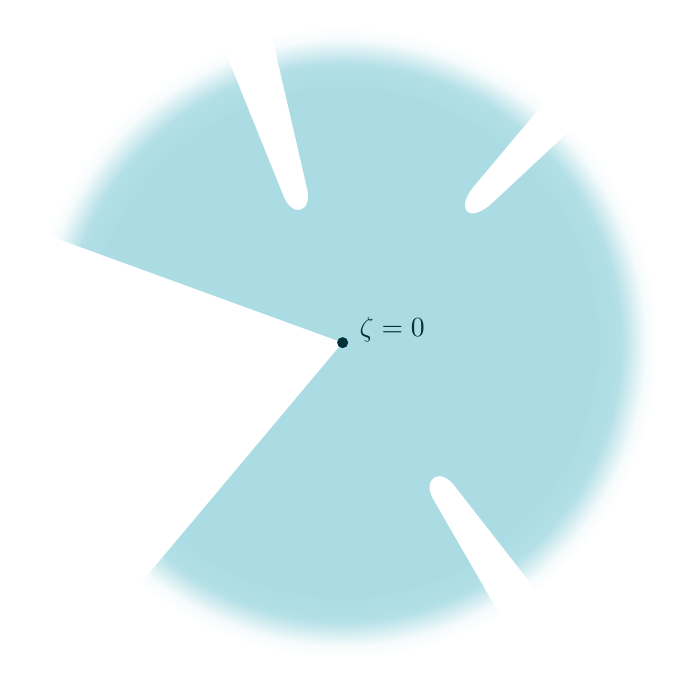
\begin{tikzpicture}
\newcommand{\spill}{4}
\fill[ietcoast!33, bezier bounding box, path fading=radial edge]
  (-\spill, -\spill) (\spill, \spill)
  (0, 0) -- (160:\spill)
  arc (160:112:\spill) -- (112:2) .. controls (112:1.7) and (103:1.7) .. (103:2) -- (103:\spill)
  arc (103:50:\spill) -- (50:2.6) .. controls (50:2.2) and (43:2.2) .. (43:2.6) -- (43:\spill)
  arc (43:-52:\spill) -- (-52:2.3) .. controls (-52:2) and (-60:2) .. (-60:2.3) -- (-60:\spill)
  arc (-60:-130:\spill) -- (0, 0);
\fill[ietcoast!33!black] circle (0.7mm) node[anchor=195, outer sep=1mm] {$\zeta = 0$};
\end{tikzpicture}
\end{center}
%
\subsubsection{The prototype operator}\label{setting:basic}
The prototypical example of the kind of operator we will be working with is a holomorphic Volterra operator $\hardpart$ with a separable kernel $\hardker$ and a regular singularity at $\zeta = 0$.

Let $\holo(\domain)$ be the space of holomorphic functions on $\domain$.
% \color{red}
% Being a holomorphic Volterra operator means that $\hardpart$ sends each holomorphic function $\varphi$ on $\domain$ to a new holomorphic function
% \[ [\hardpart\,\varphi](a) = \int_{\zeta = 0}^a \hardker(a, \cdot)\,\varphi\;d\zeta. \]
% Being separable means that the kernel $\hardker(a, a')$ factors into a function of $a$ times a function of $a'$. We will suppose this product can be written as a ratio
% \[ \hardker(a, a') = - \frac{q(a')}{p(a)}, \]
% where $p$ and $q$ are holomorphic functions on $\domain$. Having a regular singularity at $\zeta = 0$ means the following:\color{brown}
\begin{definition}\label{defn:volterra}
A {\em holomorphic Volterra operator} on $\domain$ is a linear operator
\[\genvolterra\colon\holo(\domain)\to\holo(\domain) \]
defined by an integral
\[ [\genvolterra\,\varphi](a) = \int_{\zeta = 0}^a \genker(a, \cdot)\,\varphi\;d\zeta \]
in which the {\em kernel} $w$ is a holomorphic function on $\Omega^2$.
\end{definition}
\begin{definition}
A holomorphic Volterra operator is {\em separable} if its kernel factors as a product of two functions, one on each factor of $\Omega^2$.
\end{definition}
For the prototype operator $\hardpart$, we will suppose that the kernel $\hardker$ can be written as a ratio
\[ \hardker(a, a') = - \frac{q(a')}{p(a)}, \]
for some $p, q \in \mathcal{H}(\Omega)$.

For the purposes of this paper, $\hardpart$ has a {\em regular singularity} at $\zeta=0$ if the following condition holds.

%%The Volterra operator $\hardpart$ has a regular singularity at $\zeta=0$ if the following condition holds
\begin{conditions}
\condconst{sing}{\tau}\label{cond:sing}For some constant $\tau > 0$, the difference
\[ \hardker(a, a) - \frac{\tau}{\zeta(a)} \]
is bounded on a neighborhood of $\zeta(a) = 0$ in $\domain$.
In addition, for each $\sigma > \tau$, there is a neighborhood of $\big(\zeta(a), \zeta(a')\big) = (0, 0)$ in $\Omega^2$ on which
\[ |\hardker(a, a')| < \frac{\sigma}{|\zeta(a)|}. \]
\end{conditions}
For most of our results, we will need to make sure that $\domain$ does not touch any singularities of $\hardker$ other than the one at $\zeta = 0$. We will also need to control $\hardker(a, a')$ when $a$ is away from $\zeta = 0$, requiring $\hardker$ to be bounded on the diagonal in $\domain^2$ and to grow at most exponentially as we move away from the diagonal. These requirements can be combined into one condition.
\begin{conditions}
\condconst{diag$_0$}{\lambda_\Delta}\label{cond:diag-basic} For some constant $\lambda_\Delta$, we have
\[ |\hardker(a, a')| \lesssim \frac{1}{|\zeta(a)|} e^{\lambda_\Delta|\zeta(a)-\zeta(a')|} \]
over all $a, a' \in \domain$.
\end{conditions}
This condition explains why $\domain$ \textcolor{brown}{might have the shape} illustrated in Section~\ref{setting:domain}. As $\domain$ stretches out toward infinity, it has to part around the zeros of $p$, keeping well away from every zero except the one at $\zeta = 0$.
\begin{verify}
    By Condition \eqref{cond:diag-basic} \textcolor{red}{we can find} there exists $c>0$ such that \[ | \hardker(a, a') | \le \frac{c}{|\zeta(a)|} e^{\lambda_\Delta|\zeta(a)-\zeta(a')|} \]
then setting $\delta=\frac{\log(\sigma/c)}{2\lambda_\Delta}$, we deduce that for every $|\zeta(a)|\le\delta$ and  $|\zeta(a')|\le\delta$
\begin{align*}
    |\hardker(a,a')|&\le \frac{c}{|\zeta(a)|} e^{\lambda_\Delta|\zeta(a)-\zeta(a')|}\\
    &\le \frac{c}{|\zeta(a)|} e^{\lambda_\Delta(|\zeta(a)|+|\zeta(a')|)}\\
    &\frac{c}{|\zeta(a)|} e^{2\lambda_\Delta \delta}\\
    &=\frac{\sigma}{|\zeta(a)|}
\end{align*}
\end{verify}

We will occasionally mention an optional condition on $p$ that allows us to state our main results more explicitly.
\begin{conditions}
\condconst{reg-p}{B, \epsilon}\label{cond:reg-p}
For some non-zero constant $B$ and some $\epsilon > 0$,
\[ p \in B\zeta + O\big(|\zeta|^{1 + \epsilon}\big) \]
at $\zeta = 0$.
\end{conditions}
\subsubsection{The perturbed operator}\label{setting:perturbed}

We now perturb $\hardpart$ to a more general operator $\volterra=\hardpart +\softpart$\textcolor{brown}{, where $\softpart$ has non-separable kernel, and it regularizes the action of $\softpart$ at the singularity, as we will show in Proposition \ref{prop:smoothing}.} \textcolor{blue}{The perturbation $\softpart$ will be non-separable,}\footnote{Unless $\softpart$ is zero, of course.} but it will have a regularizing effect, as we will show in Proposition \ref{prop:smoothing}. To get the smoothing effect, we will require the kernel $\softker$ of $\softpart$ to vanish to some order $\gamma > 0$ on the diagonal in $\domain^2$. This requirement, combined with two others, will be made precise in Condition~\eqref{cond:eps-lambda}.

Since $\softpart$ is a holomorphic Volterra operator, $\softker$ is a holomorphic function on $\domain^2$. We will allow $\softker(a, a')$ to have a simple pole at $\zeta(a) = 0$, like $\hardker(a, a')$ does, but we will not allow any sharper singularity. We will also put an exponential bound \textcolor{red}{on how fast $\softker$ grows away from the diagonal} \textcolor{blue}{on the growth of $\softker$ away from the diagonal}, mimicking Condition~\eqref{cond:diag-basic} on $\hardker$. Altogether, we will require:
\begin{conditions}
\condconst{diag$_\star$}{\gamma, \lambda_\Delta}\label{cond:eps-lambda} \textcolor{red}{For some constant $\gamma > 0$, we have} \textcolor{blue}{There is a constant $\gamma > 0$ for which}
\[ |\softker(a, a')| \lesssim\frac{|\zeta(a)-\zeta(a')|^\gamma}{|\zeta(a)|}\,e^{\lambda_\Delta|\zeta(a)-\zeta(a')|}\]
over all $a, a' \in \domain$.
\end{conditions}
Notice that this condition prevents $\softker$ from being separable---unless it is zero, of course.

Like $\hardker$, the combined kernel $k = \hardker + \softker$ of $\volterra$ grows in a controlled way when its arguments are near $\zeta = 0$, and when the difference between its arguments grows. We will provide specific bounds in Section~\ref{sec:bounds on k}. 

\subsection{Main results}\label{sec:results}
We want to show that when $\volterra$ is a regular singular Volterra operator of the kind described in Section~\ref{setting:perturbed}, the equation $f = \volterra f$ has a unique solution of a certain form. For the prototypical operator $\hardpart$ described in Section~\ref{setting:basic}, this solution can be written explicitly.
\begin{theorem}\label{thm:basic_volterra}
Suppose $\hardpart$ satisfies {\em Condition \eqref{cond:sing}}. Then the equation
\begin{equation}\label{eq:hardpart}
f = \hardpart f    
\end{equation}
has the {\em prototype solution}
\begin{equation}\label{eqn:test_solution}
\solproto(a) = \frac{1}{p(a)} \exp\left(-\int_{b}^{a}\frac{q}{p}\;d\zeta\right).
\end{equation}
Changing the base point $b \in \domain$ \textcolor{blue}{only} multiplies $f_0$ by a non-zero constant.
\end{theorem}
We will prove this result in Section~\ref{sec:construction}.

The solution $\solproto$ from Theorem~\ref{thm:basic_volterra} has, at worst, a mild power-law singularity at $\zeta = 0$. With stronger constraints on $\hardpart$, \textcolor{red}{we can also ensure} \textcolor{brown}{it is guaranteed} that $\solproto$ grows at most exponentially as $|\zeta| \to \infty$. The function spaces defined in Section~\ref{fn-spaces} express both of these regularity properties.
%\textcolor{Tomato}{If we change Condition \eqref{cond:sing}, it'll be enough to assume Condition \eqref{cond:diag-basic} to state Theorem \ref{thm:proto-growth}.}
\begin{theorem}\label{thm:proto-growth}
Suppose $\hardpart$ satisfies {\em Condition~\eqref{cond:sing}}. Then, on a small enough neighborhood of $\zeta = 0$, we have $|\solproto| \lesssim |\zeta|^{\tau-1}$.

Suppose $\hardpart$ also satisfies {\em Condition~\eqref{cond:diag-basic}}. Then $f_0$ belongs to the space $\singexpalg{\tau-1}(\domain)$ defined in Section~\ref{fn-spaces}.
\end{theorem}
We will prove this result in Section~\ref{sec:asymptotics}.
\begin{rmk}
When $\hardpart$ also satisfies Condition~\eqref{cond:reg-p}, we can get a better estimate of the prototype solution near $\zeta = 0$, as described in Proposition~\ref{prop:better-proto-estimate} from Section~\ref{sec:asymptotics}.
\end{rmk}
%
\textcolor{red}{When we perturb $\hardpart$ to the more general operator $\volterra = \hardpart + \softpart$ from Section~\ref{setting:perturbed}, the equation we are trying to solve gets more complicated} \textcolor{brown}{For the pertubed operator $\volterra=\hardpart+\softpart$, the equation $f=\volterra f$ is more complicated}, but its regular singularity at $\zeta = 0$ \textcolor{violet}{stays [make previous part of sentence consistent]} essentially the same. We might therefore expect to find a solution that looks like $\solproto$ near the singularity, differing only by a less singular perturbation. If we strengthen the constraints on $\hardpart$ a little more, this expectation is fulfilled.
\begin{theorem}\label{thm:general_volterra}
Suppose $\hardpart$ satisfies {\em Conditions \eqref{cond:sing}} and \eqref{cond:diag-basic}, and $\softpart$ satisfies {\em Condition~\eqref{cond:eps-lambda}}. Then the equation
\[ f = \volterra f \]
has a unique solution $f$ in the affine subspace
\[ f_0 + \singexpalg{\tau-1+\gamma}(\Omega) \]
of the space $\singexpalg{\tau-1}(\Omega)$ defined in Section~\ref{fn-spaces}. Here, $f_0$ is the prototype solution \eqref{eqn:test_solution} from Theorems \ref{thm:basic_volterra}--\ref{thm:proto-growth}, which belongs to the space $\singexpalg{\tau-1}(\domain)$.

\color{red}For any $\rho > \tau$, the uniqueness of the solution still holds in $f_0 + \singexpalg{\rho-1}(\Omega)$. In other words, lowering $\rho$ into $(\tau, \tau+\gamma)$ to allow a sharper singularity will not reveal any more solutions, and raising $\rho$ too high to admit the solution found in $f_0 + \singexpalg{\tau-1+\gamma}(\Omega)$ will leave no solution at all.\color{black}
\end{theorem}
\color{brown}
\begin{rmk}
   For any $\rho > \tau$, the uniqueness of the solution still holds in $f_0 + \singexpalg{\rho-1}(\Omega)$. In other words, lowering $\rho$ into $(\tau, \tau+\gamma)$ to allow a sharper singularity will not reveal any more solutions, and raising $\rho$ too high to admit the solution found in $f_0 + \singexpalg{\tau-1+\gamma}(\Omega)$ will leave no solution at all. \textcolor{orange}{[Place in a remark and prove in a proposition, as with the remark stating the result of Proposition~\ref{prop:alt-general_volterra}.]}
\end{rmk}
\color{black}
This result will follow from a more general result about inhomogeneous equations.
\begin{lemma}\label{lem:perturbed_volterra}
Suppose $\hardpart$ satisfies {\em Conditions \eqref{cond:sing}} and \eqref{cond:diag-basic}, and $\softpart$ satisfies {\em Condition \eqref{cond:eps-lambda}}. Suppose we are also given a function $g$, which for some $\rho > \tau$ belongs to the space $\singexpalg{\rho-1}(\Omega)$ defined in Section~\ref{fn-spaces}. Then the inhomogeneous equation
\[ f = \volterra f + g, \]
has a unique solution $f$ in the space $\singexpalg{\rho-1}(\Omega)$.
\end{lemma}
We will prove Lemma~\ref{lem:perturbed_volterra} in Sections \ref{sec:V is a contraction}--\ref{sec:existence and uniqueness}, using the contraction mapping theorem. The heart of the argument is Proposition~\ref{prop:get-contraction}, which shows us how to find relevant subspaces where $\volterra$ is a contraction.

We will reduce Theorem~\ref{thm:general_volterra} to Lemma~\ref{lem:perturbed_volterra} in Section~\ref{sec:existence and uniqueness}, by rewriting \textcolor{blue}{the homogeneous equation $f = \volterra f$ in the subspace $f_0 + \singexpalg{\tau-1+\gamma}(\Omega)$} as an inhomogeneous equation in a more regular space. To show that the inhomogeneous term, $\softpart f_0$, is regular enough, we will use Proposition~\ref{prop:smoothing} from Section~\ref{sec:image under soft_part} proving that $\softpart$ improves on the regularity of $f_0$ described by Theorem~\ref{thm:proto-growth}.
\begin{rmk}
When $\hardpart$ also satisfies Condition~\eqref{cond:reg-p}, Theorem~\ref{thm:general_volterra} can be restated to give a unique solution in the affine subspace
\[ \zeta^{\tau-1} + \singexpalg{\rho-1}(\domain) \]
when $\rho > \tau$ is \textcolor{blue!50}{low enough}, as described in Proposition~\ref{prop:alt-general_volterra} from Section~\ref{sec:existence and uniqueness}.
\end{rmk}
\subsection{Acknowledgements}
We are grateful for the conversations with Kihyun Kim, Angeliki Menegaki, and Sung-Jin Oh that informed the early stages of this work. This paper is a result of the ERC-SyG project, Recursive and Exact New Quantum Theory (ReNewQuantum) which received funding from the European Research Council (ERC) under the European Union's Horizon 2020 research and innovation programme under grant agreement No 810573. It was also made possible by the hospitality of the Institut des Hautes \'{E}tudes Scientifiques during a return visit by AF, funded by the Fondation Math\'{e}matique Jacques Hadamard under the \textit{Junior Scientific Visibility} program.
\section{Function spaces for holomorphic Volterra operators}\label{fn-spaces}
\subsection{Weighted holomorphic $L^{\infty}$ spaces}\label{sec:fn-space-defs}
Throughout this paper, as described in Section~\ref{motivation}, the position variable $\zeta$ will be the standard coordinate on $\C$. Take a simply connected open set $\domain \subset \C$ that touches but does not contain $\zeta = 0$. \textcolor{blue}{Let $\cont(\domain)$ be the space of continuous complex-valued functions on $\domain$, equipped with the compact-open topology. This} is the coarsest topology in which the seminorm $f \mapsto \sup_K |f|$ is continuous for every compact subset $K \subset \domain$~\cite[Example~2.6 and Section~4 notes]{fnl-cpx-anal}.

The holomorphic functions form a closed subspace $\holo(\domain) \subset \cont(\domain)$~\cite[Proposition~3.14]{fnl-cpx-anal}. \color{blue}We first restrict our attention to holomorphic functions on $\domain$ which are uniformly of exponential type $\Lambda \in \R$.
\begin{definition}\label{def:unif-exp}
For any $\Lambda \in \R$, let
\[ \singexp{0}{\Lambda}(\domain) \subset \holo(\domain) \]
be the subspace consisting of functions $f$ with $f \lesssim e^{\Lambda|\zeta|}$ over $\domain$, equipped with the norm
\[ \|f\|_{0, \Lambda} := \sup_\Omega e^{-\Lambda|\zeta|}\,|f|. \]
\end{definition}
With respect to the seminorm on $\holo(\domain)$ given by a compact set $K \subset \domain$, the inclusion map $\singexp{0}{\Lambda}(\domain) \hookrightarrow \holo(\domain)$ has norm $\sup_K e^{\Lambda |\zeta|}$. That means the inclusion is continuous.
%%\textcolor{orange}{$\{f \in \holo(\domain) : f \lesssim |\zeta|^\sigma e^{\Lambda|\zeta|}\}$}
\begin{rmk}
The subspace of functions of exponential type $\Lambda$ strictly contains $\singexp{0}{\Lambda}(\domain)$. A function $f$ is of exponential type $\Lambda$ if for every $\varepsilon>0$, there is a constant $A_\varepsilon$ such that $|f|\le A_\varepsilon e^{(\Lambda+\varepsilon)|\zeta|}$. Definition~\ref{def:unif-exp} instead requires a uniform constant $A$ such that $|f| \le A e^{\Lambda|\zeta|}$.\end{rmk}
We now relax our norm to allow both exponential growth at infinity and a power-law singularity at $\zeta = 0$.
\begin{definition}
For any $\sigma, \Lambda \in \R$, let
\[ \singexp{\sigma}{\Lambda}(\domain) \subset \holo(\domain) \]
be the subspace consisting of functions $f$ with $f \lesssim |\zeta|^\sigma e^{\Lambda|\zeta|}$ over $\domain$, equipped with the norm
\[ \|f\|_{\sigma,\Lambda} := \sup_\Omega |\zeta|^{-\sigma} e^{-\Lambda|\zeta|}\,|f|. \]
\end{definition}
The inclusion $\singexp{\sigma}{\Lambda}(\domain) \hookrightarrow \holo(\domain)$ is again continuous.
\begin{proposition}\label{exp-complete}
The space $\singexp{\sigma}{\Lambda}(\domain)$ is complete.
\end{proposition}
\begin{proof}
Take a Cauchy sequence $(f_j)_{j \in \N}$ in $\singexp{\sigma}{\Lambda}(\domain)$. This sequence is Cauchy in $\holo(\domain)$ as well, because the inclusion map $\singexp{\sigma}{\Lambda}(\domain) \hookrightarrow \holo(\domain)$ is bounded with respect to each of the seminorms on $\holo(\domain)$ given by $f \mapsto \sup_K |f|$ for compact subsets $K \subset \domain$. Since $\holo(\domain)$ is complete~\cite[Proposition~3.5]{fnl-cpx-anal},\footnote{That is, a sequence which is Cauchy in each of the seminorms on $\holo(\domain)$ will always converge in the topology of $\holo(\domain)$, which is the coarsest topology in which all of the seminorms are continuous.} our sequence converges to a function $f$ there.

The Cauchy property in $\singexp{\sigma}{\Lambda}(\domain)$ says that for any $r > 0$, there is some $n$ for which $|\zeta|^{-\sigma} e^{-\Lambda |\zeta|}\,|f_k - f_n| \le r$ whenever $k \ge n$. Since convergence in $\holo(\domain)$ implies pointwise convergence, it follows that $|\zeta|^{-\sigma} e^{-\Lambda |\zeta|}\,|f - f_n| \le r$. This reasoning shows that $(f_j)_{j \in \N}$ converges to $f$ in the norm $\|\cdot\|_{\sigma, \Lambda}$. It also shows that $f$ is in $\singexp{\sigma}{\Lambda}(\domain)$: picking some $r > 0$, we have
\begin{align*}
|\zeta|^{-\sigma} e^{-\Lambda |\zeta|}\,|f| & \le |\zeta|^\sigma e^{-\Lambda |\zeta|}\,|f - f_n| + |\zeta|^{-\sigma} e^{-\Lambda |\zeta|}\,|f_n| \\
& \le r + \|f_n\|_{\sigma,\Lambda}
\end{align*}
for the corresponding $n$, so $|\zeta|^{-\sigma} e^{-\Lambda |\zeta|}\,|f|$ is bounded.
\end{proof}
\color{black}
\subsection{Continuous inclusions between different $\singexp{\sigma}{\Lambda}(\Omega)$}\label{sec:inclusions}
\begin{proposition}\label{prop:inclus-ge-exp}
If $\Lambda'\leq\Lambda$, the inclusion map $\singexp{\sigma}{\Lambda'}(\Omega)\hookrightarrow \singexp{\sigma}{\Lambda}(\Omega)$ is continuous.
\end{proposition}
\begin{proof}
By definition,
\[ \|f\|_{\sigma,\Lambda}=\sup_{\Omega} |\zeta|^{-\sigma}\,e^{-\Lambda |\zeta|}\, |f|. \]
The norm $\|\cdot\|_{\sigma, \Lambda'}$ is designed to give $|f| \le |\zeta|^\sigma\,e^{\Lambda'|\zeta|}\,\|f\|_{\sigma, \Lambda'}$, implying that
\begin{align*}
\|f\|_{\sigma,\Lambda} & \leq \sup_{\Omega} |\zeta|^{-\sigma}\,e^{-\Lambda |\zeta|}\,|\zeta|^\sigma\,e^{\Lambda'|\zeta|}\,\|f\|_{\sigma, \Lambda'}\\
&=\sup_{\Omega} e^{-(\Lambda-\Lambda') |\zeta|}\,\|f\|_{\sigma, \Lambda'}\\
&\leq \|f\|_{\sigma,\Lambda'}.
\end{align*}
In the last step, we use the assumption that $\Lambda' \le \Lambda$.
\end{proof}
%\textcolor{blue}{One might describe the functions in $\singexp{\sigma}{\Lambda}(\domain)$ as being uniformly of exponential type $\Lambda$.\footnote{Recall that a function $f$ is of exponential type $\Lambda$ if for every $\varepsilon>0$, there is a constant $A_\varepsilon$ (which may depends on $\varepsilon$) such that $|f|\le A_\varepsilon e^{(\Lambda+\varepsilon)|\zeta|}$. We instead require a uniform constant $A$ such that $|f| \le A e^{\Lambda|\zeta|}$.}
\color{blue}

The union $\bigcup_{\Lambda \in \R} \singexp{0}{\Lambda}(\domain)$ is the subspace comprising all functions of exponential type. The continuous inclusions between the $\singexp{0}{\Lambda}(\domain)$ define a limit topology on this subspace. The spaces $\singexp{\sigma}{\Lambda}(\domain)$ fit together analogously for other $\sigma \in \R$.
\begin{definition}\label{def:exp-top}
For any $\sigma \in \R$, let $\singexpalg{\sigma}(\domain)$ be the union
\[ \bigcup_{\Lambda \in \R} \singexp{\sigma}{\Lambda}(\domain) \]
equipped with the finest topology that makes all the inclusions $\singexp{\sigma}{\Lambda}(\domain) \hookrightarrow \singexpalg{\sigma}(\domain)$ continuous.
\end{definition}
\color{brown}
\begin{definition}
    Let $\sigma \in \R$. We define the space
    \[\singexpalg{\sigma}(\domain):=\bigcup_{\Lambda\in\R}\singexp{\sigma}{\Lambda}(\domain)\,,\]
    equipped with the finest topology that makes continuous the inclusions $\singexp{\sigma}{\Lambda}(\domain) \hookrightarrow \singexpalg{\sigma}(\domain)$. 
\end{definition}
\color{red} Taking the union of these spaces over all $\Lambda \in \R$, we get the space $\singexpalg{0}(\domain)$ that contains all functions of exponential type. Having continuous inclusions between the subspaces $\singexp{0}{\Lambda}(\domain)$ as $\Lambda$ increases, we \textcolor{red}{can} give $\singexpalg{0}(\domain)$ a meaningful topology: the finest topology that makes all the inclusions $\singexp{0}{\Lambda}(\domain) \hookrightarrow \singexpalg{0}(\domain)$ continuous.\footnote{In category-theoretic language, $\singexpalg{0}(\domain)$ is the limit of the family $\singexp{0}{\Lambda}(\domain)$.} For any $\sigma \in \R$, we define $\singexpalg{\sigma}(\domain)$ similarly.
\color{black}
\begin{proposition}\label{prop:inclus-lt-pow-gt-exp}
If $\sigma'>\sigma$ and $\Lambda'<\Lambda$, the inclusion map $\singexp{\sigma'}{\Lambda'}(\Omega)\hookrightarrow \singexp{\sigma}{\Lambda}(\Omega)$ is continuous.
\end{proposition}
\begin{proof}
By definition,
\begin{align*}
\|f\|_{\sigma,\Lambda}&=\sup_{\Omega} |\zeta|^{-\sigma}  e^{-\Lambda |\zeta|} |f|\\
&= \sup_{\Omega} |\zeta|^{\sigma'-\sigma}\,|\zeta|^{-\sigma'}\,e^{-\Lambda'|\zeta|}\,  e^{-(\Lambda-\Lambda') |\zeta|} \, |f|.
\end{align*}
The function $|\zeta|^{\sigma'-\sigma}\,  e^{-(\Lambda-\Lambda') |\zeta|}$ is bounded near $\zeta = 0$ because the power of $|\zeta|$ is positive, and it is bounded far from $\zeta = 0$ thanks to the decaying exponential. Hence,
\begin{align*}
\|f\|_{\sigma,\Lambda}&\leq C\sup_\Omega  |\zeta|^{-\sigma'}\, e^{-\Lambda'|\zeta|} \, |f|\\
&=C \|f\|_{\sigma',\Lambda'}
\end{align*}
for $C = \sup_{\Omega}  |\zeta|^{\sigma'-\sigma}\,  e^{-(\Lambda-\Lambda') |\zeta|}$.
\end{proof}
\begin{proposition}\label{prop:inclus-lt-pow-alg}
When $\sigma' > \sigma$, there is a continuous inclusion $\singexpalg{\sigma'}(\domain)\hookrightarrow \singexpalg{\sigma}(\domain)$.
\end{proposition}
\color{blue}
\begin{proof}
For each $\Lambda'$, we define a continuous inclusion $\singexp{\sigma'}{\Lambda'}(\domain) \hookrightarrow \singexpalg{\sigma}(\domain)$ by choosing some $\Lambda > \Lambda'$ and composing the continuous inclusions
\begin{center}
\begin{tikzcd}[column sep=25mm, labels={inner sep=0.75ex}]
\singexp{\sigma'}{\Lambda'}(\domain) \arrow[r, hook, "\text{\footnotesize Proposition~\ref{prop:inclus-lt-pow-gt-exp}}"'] & \singexp{\sigma}{\Lambda}(\domain) \arrow[r, hook, "\text{\footnotesize Definition~\ref{def:exp-top}}"'] & \singexpalg{\sigma}(\domain).
\end{tikzcd}
\end{center}
For any $\Lambda'' < \Lambda'$, the inclusions
\begin{center}
\begin{tikzcd}[row sep=6mm, column sep=8mm, labels={inner sep=0.75ex}]
\singexp{\sigma'}{\Lambda''}(\domain) \arrow[rr, hook, "\text{\footnotesize Proposition~\ref{prop:inclus-ge-exp}}"] \arrow[rd, hook] & & \singexp{\sigma'}{\Lambda'}(\domain) \arrow[ld, hook] \\
& \singexpalg{\sigma}(\domain)
\end{tikzcd}
\end{center}
%%\begin{center}
%%\begin{tikzcd}[row sep=2mm, column sep=15mm, labels={inner sep=1ex,}]
%%\singexp{\sigma'}{\Lambda'}(\Omega) \arrow[rd, hook] \\
%%& \singexpalg{\sigma}(\Omega) \\
%%\singexp{\sigma'}{\Lambda''}(\Omega) \arrow[ru, hook] \arrow[uu, hook, "\text{\footnotesize Proposition~\ref{prop:inclus-ge-exp}}"]
%%\end{tikzcd}
%%\end{center}
automatically commute, because as non-topological linear maps they are all inclusions between subspaces of $\holo(\domain)$. The existence of the desired continuous inclusion $\singexpalg{\sigma'}(\Omega)\hookrightarrow \singexpalg{\sigma}(\Omega)$ then follows from the universal property of the limit topology.
\par\color{red}
For each $\Lambda'$, we \textcolor{red}{can} get a continuous inclusion $\singexp{\sigma'}{\Lambda'}(\Omega) \hookrightarrow \singexpalg{\sigma}(\Omega)$ by choosing \textcolor{red}{some} $\Lambda > \Lambda'$ and composing the continuous inclusion $\singexp{\sigma'}{\Lambda'}(\Omega) \hookrightarrow \singexp{\sigma}{\Lambda}(\Omega)$ given by Proposition~\ref{prop:inclus-lt-pow-gt-exp} with the continuous inclusion $\singexp{\sigma}{\Lambda}(\Omega) \hookrightarrow \singexpalg{\sigma}(\Omega)$ that we get by definition. For any $\Lambda'' < \Lambda'$, the inclusions $\singexp{\sigma'}{\Lambda''}(\Omega) \hookrightarrow \singexpalg{\sigma}(\Omega)$ and $\singexp{\sigma'}{\Lambda'}(\Omega) \hookrightarrow \singexpalg{\sigma}(\Omega)$ constructed above automatically commute with the inclusion $\singexp{\sigma'}{\Lambda''}(\Omega) \hookrightarrow \singexp{\sigma'}{\Lambda'}(\Omega)$ given by Proposition~\ref{prop:inclus-ge-exp}, because we are ultimately working in the vector space of holomorphic functions on $\Omega$. Because of how the topology on $\singexpalg{\sigma'}(\Omega)$ is defined, this gives us the desired continuous inclusion $\singexpalg{\sigma'}(\Omega)\hookrightarrow \singexpalg{\sigma}(\Omega)$.
\par\color{brown}
For every $\Lambda'$, there is a continuous inclusion $\singexp{\sigma'}{\Lambda'}(\Omega) \hookrightarrow \singexpalg{\sigma}(\Omega)$ obtained by choosing $\Lambda > \Lambda'$ and composing the continuous inclusion $\singexp{\sigma'}{\Lambda'}(\Omega) \hookrightarrow \singexp{\sigma}{\Lambda}(\Omega)$ given by Proposition~\ref{prop:inclus-lt-pow-gt-exp} with the continuous inclusion $\singexp{\sigma}{\Lambda}(\Omega) \hookrightarrow \singexpalg{\sigma}(\Omega)$.

For any $\Lambda'' < \Lambda'$, the inclusions $\singexp{\sigma'}{\Lambda''}(\Omega) \hookrightarrow \singexpalg{\sigma}(\Omega)$ and $\singexp{\sigma'}{\Lambda'}(\Omega) \hookrightarrow \singexpalg{\sigma}(\Omega)$ constructed above automatically commute with the inclusion $\singexp{\sigma'}{\Lambda''}(\Omega) \hookrightarrow \singexp{\sigma'}{\Lambda'}(\Omega)$ given by Proposition~\ref{prop:inclus-ge-exp}, because we are working in the space of holomprhic functions on $\domain$. In the topology of $\singexpalg{\sigma'}(\domain)$, this gives the desired continuos inclusion $\singexpalg{\sigma'}(\Omega)\hookrightarrow \singexpalg{\sigma}(\Omega)$.
\color{black}
\end{proof}
\section{Solving holomorphic Volterra equations}\label{sec:proof_main_results}
\subsection{Overview}
\color{blue}
In this section, we prove the results stated in Section~\ref{sec:results}, which lay out a method for solving the regular singular Volterra equation $\solwhole = \volterra \solwhole$.

We first construct the prototype solution $\solproto$ from the kernel of $\hardpart$. We show in Section~\ref{sec:proto-construction-regularity} that $\solproto$ satisfies the equation $\solproto = \hardpart \solproto$ and belongs to the space $\singexp{\tau-1}{\lambda_0}(\domain)$.

We then study how the perturbation $\softpart$ affects $\solproto$. We show in Section~\ref{sec:image under soft_part} that $\softpart$ has a smoothing effect, reducing the sharpness of any power-law singularity at $\zeta = 0$. In particular, it sends $\solproto$ into $\singexpalg{\tau-1+\gamma}(\domain)$.
\par\textcolor{orange}{[Keep revising]} \color{red}
The results stated in Section~\ref{sec:results} lay out a method for solving the regular singular Volterra equation $\solwhole = \volterra \solwhole$. In this section, we show that the method works by proving those results.

We start by constructing the prototype solution $\solproto$ from the kernel of $\hardpart$, which is the separable operator that gives $\volterra = \hardpart + \softpart$ its regular singularity. We will show in Section~\ref{sec:proto-construction-regularity} that $\solproto$ satisfies the equation $\solproto = \hardpart \solproto$ and belongs to the space $\singexp{\tau-1}{\lambda_0}(\domain)$.

To see what the perturbation $\softpart$ does to $\solproto$, we will show in Section~\ref{sec:image under soft_part} that $\softpart$ has a smoothing effect, reducing the sharpness of any power-law singularity at $\zeta = 0$. In particular, it sends $\solproto$ into $\singexpalg{\tau-1+\gamma}(\domain)$.

\color{brown}
In this section, we prove the results outlined in Section~\ref{sec:results}, demonstrating a method for solving the singular Voletrra equation $f=\volterra f$. 

We start by constructing the prototype solution $f_0$ of $f=\softpart f$, and show in Section~\ref{sec:proto-construction-regularity} that $f_0\in\singexp{\tau-1+\gamma}{\Lambda}(\domain)$. 

In Section~\ref{sec:image under soft_part}, we show that the perturbation $\softpart$ has a smoothing effect on $f_0$, reducing the power-law singularity at $\zeta=0$. In particular, it turns out that $\softpart f_0\in\singexpalg{\tau-1+\gamma}(\domain)$.
\color{black}

\textcolor{red}{Now we know that} \textcolor{brown}{Therefore} $\volterra$ sends $\solproto$ into the affine subspace $\solproto + \singexpalg{\tau-1+\gamma}(\domain)$, suggesting that the equation $\solwhole = \volterra \solwhole$ has a solution there. To confirm this, we will show in Section~\ref{sec:V is a contraction} that $\volterra$ is a contraction of $\singexp{\tau-1+\gamma}{\Lambda}(\domain)$ when $\Lambda$ is large enough. This implies that $\volterra$ has a unique fixed point in $\solproto + \singexpalg{\tau-1+\gamma}(\domain)$, as we will see in Section~\ref{sec:existence and uniqueness}.
\subsection{Construction and regularity of the prototype solution \\ \textit{(proof of Theorems~\ref{thm:basic_volterra}--\ref{thm:proto-growth})}}\label{sec:proto-construction-regularity}
\subsubsection{Construction}\label{sec:construction}
\begin{proof}[Proof of Theorem~\ref{thm:basic_volterra}]
Rewrite $\solproto$ as $(1/p)\,\chi$, where
\[ \chi(a) = \exp\left(-\int_{b}^{a}\frac{q}{p}\;d\zeta\right). \]
Observing that $d\chi = -(q/p)\,\chi\;d\zeta$ \textcolor{blue}{simplifies} the calculation of $\hardpart \solproto$. For each $a \in \domain$,
\begin{align*}
\big[\hardpart \solproto\big](a) &= - \int_{\zeta=0}^{a} \frac{q}{p(a)}\,\solproto\;d\zeta \\
& = -\int_{\zeta=0}^{a} \frac{q}{p(a)}\,\frac{1}{p}\,\chi\;d\zeta \\
& = - \frac{1}{p(a)}  \int_{\zeta=0}^{a} \frac{q}{p}\,\chi\;d\zeta\\
& = \frac{1}{p(a)} \int_{\zeta=0}^{a}\;d\chi \\
& = \frac{1}{p(a)} \left[ \chi(a) - \lim_{\zeta \to 0} \chi \right] \\
& = \solproto(a) - \frac{1}{p(a)} \lim_{\zeta \to 0} \chi.
\end{align*}
\textcolor{blue}{To prove that $\hardpart \solproto = \solproto$, we must now} show that $\lim_{\zeta \to 0} \chi = 0$.

By Condition~\eqref{cond:sing}, \textcolor{blue}{there exist} a radius $\delta>0$ and a constant $C$ such that
\begin{equation}\label{eqn:sing-bound}
\left|\frac{q}{p} + \frac{\tau}{\zeta}\right| < C
\end{equation}
whenever $|\zeta| < \delta$. \textcolor{blue}{To use this bound, we rewrite the integral in the definition of $\chi$:} \textcolor{red}{We can take advantage of} \textcolor{magenta}{We use this bound [we do not use the bound yet]} \textcolor{pink}{by rewriting the integral in the definition of $\chi$:}
\begin{align*}
-\int_b^a \frac{q}{p}\;d\zeta & = \int_b^a \frac{\tau}{\zeta}\;d\zeta - \int_b^a \left( \frac{q}{p} + \frac{\tau}{\zeta} \right)\;d\zeta \\
& = \tau \log\left(\frac{\zeta(a)}{\zeta(b)}\right) - \int_b^a \left( \frac{q}{p} + \frac{\tau}{\zeta} \right)\;d\zeta
\end{align*}
Exponentiating both sides, we see that
\[ \chi(a) = \left(\frac{\zeta(a)}{\zeta(b)}\right)^\tau \exp\left[-\int_b^a \left( \frac{q}{p} + \frac{\tau}{\zeta} \right)\;d\zeta\right]. \]
Recalling that a change of base point just multiplies $\solproto$ by a non-zero constant, choose the base point $b \in \Omega$ so that $|\zeta(b)| = \delta/2$. The exponential factor in the formula above is then bounded between $\exp\big({-\tfrac{3}{2}C\delta}\big)$ and $\exp\big(\tfrac{3}{2}C\delta\big)$ whenever $|\zeta(a)| < \delta$. Since $\tau$ is positive, this is enough to show that $\lim_{\zeta \to 0} \chi = 0$. It follows, as discussed above, that $\hardpart \solproto = \solproto$. 
\color{orange}
For $\tau\in\C$
\begin{equation}
    \left(\frac{\zeta(a)}{\zeta(b)}\right)^\tau=\exp\left(\Re(\tau) \textcolor{magenta}{\log} \frac{\zeta(a)}{\zeta(b)}+i\Im(\tau)\textcolor{magenta}{\log} \frac{\zeta(a)}{\zeta(b)}\right)
\end{equation}
so if $\Re(\tau)>0$ and it is bigger than $\Im(\tau)$ the first term dominates in the limit $\zeta\to0$...but maybe we don't need ``bigger than $\Im(\tau)$", as ``we can rotate". I'm not very confortable with rotations, so probably I'll not add this complication. I'm also afraid we should be more carefull with these mooving domains, if we allow rotations. So maybe better not make things too complicated for the sake of generality. We have a good list of examples that fit in our pictures. 
\color{black}
\end{proof}
\subsubsection{Regularity}\label{sec:asymptotics}
%\textcolor{Tomato}{If we change Condition \eqref{cond:sing}, then we might simply have proof of Theorem \ref{thm:proto-growth} assuming only Condition \eqref{cond:diag-basic}. The proofs of the Proposition below can be combined together.}
Theorem~\ref{thm:proto-growth} comprises two results with different conditions. We will prove them separately as Propositions \ref{prop:asymptotic at zero} and \ref{prop:asymptotic at infinity}.
\begin{proposition}\label{prop:asymptotic at zero}
Suppose $\hardpart$ satisfies {\em Condition~\eqref{cond:sing}}. Then, on a small enough neighborhood of $\zeta = 0$, we have $|\solproto| \lesssim |\zeta|^{\tau-1}$.
\end{proposition}

\begin{proof}
Go back to the proof of Theorem~\ref{thm:basic_volterra}, where we found a radius $\delta > 0$ and a constant $C$ such that inequality~\eqref{eqn:sing-bound} holds whenever $|\zeta| < \delta$. The subsequent argument, which we used to show that $\lim_{\zeta \to 0} \chi = 0$, actually supports a stronger conclusion: it shows that $|\chi| \lesssim |\zeta|^\tau$ on the region $|\zeta| < \delta$. This implies that
\[ |\solproto| \lesssim \left|\frac{1}{p}\right|\,|\zeta|^\tau \]
on the region $|\zeta| < \delta$.

Now, using Condition~\eqref{cond:sing} again, \textcolor{red}{choose some $\sigma > \tau$ and find a radius $r < \delta$} for a given $\sigma>0$ there exists a radius $r<\delta$ for which
\[ \left|\frac{q(a')}{p(a)}\right| < \frac{\sigma}{|\zeta(a)|} \]
whenever $|\zeta(a)| < r$ and $|\zeta(a')| < r$. Choosing a point $b'$ with $|\zeta(b')| < r$ and $q(b') \neq 0$, we \textcolor{red}{can} deduce that
\begin{align*}
|\solproto| & \lesssim \left|\frac{1}{q(b')}\right|\,\left|\frac{q(b')}{p}\right|\,|\zeta|^\tau \\
& \lesssim \left|\frac{1}{q(b')}\right|\,\frac{\sigma}{|\zeta|}\,|\zeta|^\tau \\
& \lesssim |\zeta|^{\tau-1}
\end{align*}
on the region $|\zeta| < r$, as desired.
\end{proof}
\begin{proposition}\label{prop:asymptotic at infinity}
Suppose $\hardpart$ satisfies {\em Conditions \eqref{cond:sing}} and \eqref{cond:diag-basic}. Then $\solproto$ belongs to the space $\singexpalg{\tau-1}(\domain)$.
\end{proposition}
\begin{proof}
We want to show that $|\solproto| \lesssim |\zeta|^{\tau-1} e^{\lambda_0|\zeta|}$ for some real constant $\lambda_0$.

By Proposition~\ref{prop:asymptotic at zero}, \textcolor{blue}{there is} a radius $\delta > 0$ for which $|\solproto| \lesssim |\zeta|^{\tau-1}$ over the region $|\zeta| < \delta$. No matter which value of $\lambda_0$ we pick, \textcolor{blue}{$e^{\lambda_0|\zeta|}$ cannot get arbitrarily close to zero on a bounded region, so} $|\solproto| \lesssim |\zeta|^{\tau-1} e^{\lambda_0|\zeta|}$ over the region $|\zeta| < \delta$.

By Condition~\eqref{cond:diag-basic}, we have
\begin{align*}
|\hardker(a, a')| & \lesssim \frac{1}{|\zeta(a)|} e^{\lambda_\Delta |\zeta(a) - \zeta(a')|} \\
& \lesssim \delta^{-1} e^{\lambda_\Delta |\zeta(a) - \zeta(a')|} \\
& \lesssim e^{\lambda_\Delta |\zeta(a) - \zeta(a')|}
\end{align*}
over all $a, a' \in \domain$ with $|\zeta(a)| \ge \delta$. \textcolor{blue}{The last bound means that for some $c_\Delta > 0$,}
\[ |\hardker(a, a')| \le c_\Delta e^{\lambda_\Delta |\zeta(a) - \zeta(a')|} \]
whenever $|\zeta(a)| \ge \delta$. Applying this bound along the diagonal in $\domain^2$, we \textcolor{blue}{conclude} that $|q/p| \le c_\Delta$ on the region $|\zeta| \ge \delta$. On the other hand, by fixing some arbitrary  $b' \in \domain$, we see that
\begin{align*}
\left|\frac{q(b')}{p(a)}\right| & \lesssim \frac{1}{|\zeta(a)|} e^{\lambda_\Delta|\zeta(a) - \zeta(b')|} \\
& \lesssim \frac{1}{|\zeta(a)|} e^{\lambda_\Delta(|\zeta(a)| + |\zeta(b')|)} \\
& \lesssim \frac{1}{|\zeta(a)|} e^{\lambda_\Delta|\zeta(a)|} e^{\lambda_\Delta|\zeta(b')|} \\
& \lesssim \frac{1}{|\zeta(a)|} e^{\lambda_\Delta|\zeta(a)|}
\end{align*}
over all $a \in \domain$ with $|\zeta(a)| \ge \delta$. Using both of the bounds we just found, we \textcolor{red}{reason} deduce that
\begin{align*}
|\solproto(a)| & = \left| \frac{1}{p(a)} \exp\left(-\int_{b}^{a}\frac{q}{p}\;d\zeta\right) \right| \\
& \le \left|\frac{1}{p(a)}\right| \exp\left(\int_{b}^{a}\left|\frac{q}{p}\right|\;d\zeta\right) \\
& \lesssim \frac{1}{|\zeta(a)|} e^{\lambda_\Delta|\zeta(a)|}\,e^{c_\Delta(|\zeta(a)| + |\zeta(b)|)} \\
& \lesssim \frac{1}{|\zeta(a)|} e^{(\lambda_\Delta + c_\Delta)|\zeta(a)|}\,e^{c_\Delta|\zeta(b)|}
\end{align*}
over all $a \in \domain$ with $|\zeta(a)| \ge \delta$. Setting $\lambda_0 = \lambda_\Delta + c_\Delta$, we have $|\solproto| \lesssim |\zeta|^{-1} e^{\lambda_0|\zeta|}$ over the region $|\zeta| \ge \delta$. Since we are assuming $\tau$ is real and positive, $|\zeta|^\tau$ cannot get arbitrarily close to zero on the region $|\zeta| > \delta$. It follows that $|\solproto| \lesssim |\zeta|^{\tau-1} e^{\lambda_0|\zeta|}$ over the region $|\zeta| \ge \delta$. Combining this with our earlier argument on the region $|\zeta| < \delta$, we get the desired result.
\end{proof}
\begin{proposition}\label{prop:better-proto-estimate}
Suppose $\hardpart$ satisfies {\em Conditions~\eqref{cond:reg-p}} and \eqref{cond:sing}. Then\textcolor{red}{, for some constant $M$} \textcolor{blue}{there is some $M\in\C$} for which,
\[ \solproto \in M\zeta^{\tau-1} + O(|\zeta|^{\tau-1+\epsilon'}) \]
at $\zeta = 0$, where $\epsilon'=\min\{\epsilon, 1\}$.
\end{proposition}
\begin{proof}
It is enough to show that
\[ \solproto \in M\zeta^{\tau-1} \Big[1 + O\big(|\zeta|^{\epsilon'}\big)\Big] \]
at $\zeta = 0$. \textcolor{blue}{As in} the proof of Theorem~\ref{thm:basic_volterra}, we \textcolor{blue}{compute}
\begin{align*}
\solproto(a)&=\frac{1}{p(a)}\, \exp\left(-\int_b^a\frac{q}{p} d\zeta\;\right)\\
& = \frac{1}{p(a)}\,\frac{\zeta(a)^{\tau}}{\zeta(b)^{\tau}}\,\exp\left[-\int_b^a \left(\frac{q}{p}+\frac{\tau}{\zeta}\right) d\zeta\right]\\
& = \zeta(b)^{-\tau}\,\zeta(a)^{\tau-1}\,\frac{\zeta(a)}{p(a)} \exp\left[-\int_b^a\left(\frac{q}{p}+\frac{\tau}{\zeta}\right) d\zeta\right].
\end{align*}
\textcolor{blue}{Note that $\zeta(b)^{-\tau}$ is a constant, which will eventually be absorbed into $M$.}
\textcolor{pink}{Since $\zeta(b)^{-\tau}$ is a constant, \textcolor{red}{the $\zeta(b)^{-\tau}\,\zeta^{\tau-1}$ factor looks like what we want} the factor $\zeta(b)^{-\tau}\,\zeta^{\tau-1}$ is proportional to $\zeta^{\tau-1}$.}

\textcolor{red}{With a little work, the $\zeta/p$ factor also looks like what we want.} \textcolor{pink}{Then,} Condition \eqref{cond:reg-p} implies that
\[ \frac{\zeta}{p} \in B^{-1} + O\big(|\zeta|^{\epsilon}\big), \]
at $\zeta = 0$.

Now, let us look at the exponential factor. By Condition~\eqref{cond:sing}, \textcolor{red}{we can find} \textcolor{brown}{there exist} a constant $C$ and a neighborhood $\domain_\text{near}$ of $\zeta = 0$ for which
\[ \left| \frac{q}{p}+\frac{\tau}{\zeta} \right| < C \]
in $\domain_\text{near}$. It follows that the improper integral
\[ \eta(a) = \int_{\zeta = 0}^a \left(\frac{q}{p}+\frac{\tau}{\zeta}\right) d\zeta \]
converges for all $a \in \domain$, allowing us to write
\[ \exp\left[-\int_b^a\left(\frac{q}{p}+\frac{\tau}{\zeta}\right) d\zeta\right] = e^{\eta(b)} e^{-\eta(a)}. \]
Observing that $|\eta| \le C |\zeta|$ in $\near$, we \textcolor{red}{can} conclude that
\[ \exp\left[-\int_b^a\left(\frac{q}{p}+\frac{\tau}{\zeta}\right) d\zeta\right] \in e^{\eta(b)} \Big[ 1 + O\big(|\zeta(a)|\big) \Big] \]
at $\zeta(a) = 0$.

\textcolor{blue}{Together, the arguments above show that}\textcolor{pink}{Combining the arguments above, we \textcolor{red}{learn} \textcolor{blue}{find} that}
\begin{align*}
\solproto & \in \zeta(b)^{-\tau}\,\zeta^{\tau-1}\;\Big[ B^{-1} + O\big(|\zeta|^{\epsilon}\big) \Big]\;e^{\eta(b)} \Big[1 + O\big(|\zeta|\big) \Big] \\
& = \zeta(b)^{-\tau} B^{-1} e^{\eta(b)}\;\zeta^{\tau-1} \Big[ 1 + O\big(|\zeta|^{\epsilon}\big) \Big] \Big[1 + O\big(|\zeta|\big) \Big] \\
& = M\zeta^{\tau-1} \Big[ 1 + O\big(|\zeta|^{\epsilon}\big) + O\big(|\zeta|\big) \Big]
\end{align*}
at $\zeta = 0$, with $M = \zeta(b)^{-\tau} B^{-1} e^{\eta(b)}$. Observing that $O\big(|\zeta|^{\epsilon}\big) + O\big(|\zeta|\big) = O\big(|\zeta|^{\epsilon'}\big)$, we \textcolor{blue}{reach} the desired result.
\end{proof}
\subsection{Showing that $\softpart$ makes the prototype solution less singular \\ \textit{(toward Theorem~\ref{thm:general_volterra})}}\label{sec:image under soft_part}
Now that we know the prototype solution $\solproto$ belongs to $\singexpalg{\tau-1}(\domain)$, we will show that $\softpart$ reduces the sharpness of its singularity at $\zeta = 0$, mapping it into $\singexpalg{\tau-1+\gamma}(\domain)$. This is a consequence of the general smoothing effect of $\softpart$, described in the following result.

\begin{proposition}\label{prop:smoothing}
Under {\em Condition~\eqref{cond:eps-lambda}}, the operator $\softpart$ maps
\[ \singexp{\sigma}{\Lambda}(\Omega) \to \singexp{\sigma+\gamma}{\Lambda}(\Omega) \]
continuously for all $\Lambda\geq \lambda_{\Delta}$ and $\sigma>-1$.
\end{proposition}
\begin{rmk}
We assume $\gamma > 0$, but this result holds even under the weaker assumption that $\gamma > -1$. We will take advantage of this in Section~\ref{sec:L-int-op}
\end{rmk}
\begin{proof}[Proof of Proposition~\ref{prop:smoothing}]
For any function $f\in\singexp{\sigma}{\Lambda}(\domain)$,
\begin{align*}
|\zeta(a)|^{-(\sigma+\gamma)} \, e^{-\Lambda |\zeta(a)|} \, \Big \vert \big[ \softpart f\big](a)\Big\vert
&\leq |\zeta(a)|^{-(\sigma+\gamma)}\, e^{-\Lambda |\zeta(a)|} \int_{\zeta=0}^a |\softker(a,\cdot)|\, |f| \, |d\zeta| \\
&\leq |\zeta(a)|^{-(\sigma+\gamma)}\, e^{-\Lambda |\zeta(a)|} \int_{\zeta=0}^a |\softker(a,\cdot)|\, |\zeta|^{\sigma}\, e^{\Lambda |\zeta|} \|f\|_{\sigma,\Lambda} \, |d\zeta| 
\end{align*}
By Condition~\eqref{cond:eps-lambda},
\begin{align*}
\int_{\zeta=0}^a |\softker(a,\cdot)|\, |\zeta|^{\sigma}\, e^{\Lambda |\zeta|} \, |d\zeta| &\lesssim \int_{\zeta=0}^a \frac{|\zeta(a)-\zeta|^\gamma}{|\zeta(a)|} e^{\lambda_\Delta |\zeta(a)-\zeta|} |\zeta|^{\sigma}\, e^{\Lambda|\zeta|}\;|d\zeta|\\
&\lesssim |\zeta(a)|^{\gamma+\sigma} \int_{0}^1 (1-t)^\gamma e^{\lambda_\Delta |\zeta(a)|(1-t)} t^{\sigma}\, e^{\Lambda|\zeta(a)| t}\;dt\\
&\lesssim |\zeta(a)|^{\gamma+\sigma}\, e^{\lambda_\Delta |\zeta(a)|}\,  \int_{0}^1 (1-t)^\gamma  t^{\sigma}\,e^{(\Lambda-\lambda_\Delta)|\zeta(a)| t}\;dt\\
&\lesssim |\zeta(a)|^{\gamma+\sigma}\, e^{\lambda_\Delta |\zeta(a)|}\,e^{(\Lambda-\lambda_\Delta)|\zeta(a)|}\int_{0}^1 (1-t)^\gamma  t^{\sigma}\;dt.
\end{align*}
The last step takes advantage of the assumption that $\Lambda \ge \lambda_\Delta$. \textcolor{red}{Recognizing the integral as an evaluation of the beta function, we \textcolor{red}{can} rewrite the bound as} \textcolor{brown}{The integral defines Euler's beta function, so} \textcolor{blue}{The integral on the last line is Euler's beta integral~\cite[equation~5.12.1]{dlmf}, so}
\[ \int_{\zeta=0}^a |\softker(a,\cdot)|\, |\zeta|^{\sigma}\, e^{\Lambda |\zeta|} \, |d\zeta| \lesssim |\zeta(a)|^{\gamma+\sigma}\, e^{\Lambda |\zeta(a)|} \frac{\Gamma(\gamma+1)\Gamma(\sigma+1)}{\Gamma(\sigma+\gamma+2)}. \]
\textcolor{red}{Our assumptions that $\gamma > 0$ and $\sigma > -1$ ensure that} \textcolor{blue}{Since $\gamma > 0$ and $\sigma > -1$,} the gamma functions are well-defined.\footnote{We could even weaken the constraint on $\gamma$, allowing any $\gamma > -1$.} Rearranging to get
\[ |\zeta(a)|^{-(\gamma+\sigma)}\, e^{-\Lambda |\zeta(a)|} \int_{\zeta=0}^a |\softker(a,\cdot)|\, |\zeta|^{\sigma}\, e^{\Lambda |\zeta|} \, |d\zeta| \lesssim \frac{\Gamma(\gamma+1)\Gamma(\sigma+1)}{\Gamma(\sigma+\gamma+2)}, \]
we conclude that $|\zeta(a)|^{-\sigma-\gamma} \, e^{-\Lambda |\zeta(a)|} \, \Big \vert \big[ \softpart f\big](a)\Big\vert$ is uniformly bounded in $\domain$. 
\end{proof}
\begin{corollary}\label{cor:pertub_f0}
Consider the prototype solution $\solproto$ from Equation~\eqref{eqn:test_solution}. If $\softpart$ satisfies {\em Condition \eqref{cond:eps-lambda}}, then $\softpart \solproto$ belongs to $\singexpalg{\tau-1+\gamma}(\domain)$.
\end{corollary}
\begin{proof}
We know from Theorem~\ref{thm:proto-growth} that $\solproto$ belongs to $\singexpalg{\tau-1}(\domain)$. Choose a constant $\Lambda \ge \lambda_\Delta$ big enough that $\solproto$ is in $\singexp{\tau-1}{\Lambda}(\domain)$. Since we are assuming $\tau$ is positive, we can apply Proposition~\ref{prop:smoothing}, concluding that $\softpart \solproto$ belongs to $\singexp{\tau-1+\gamma}{\Lambda}(\domain)$.
\end{proof}
\subsection{Showing that $\volterra$ shrinks less singular functions \\ \textit{(toward Lemma~\ref{lem:perturbed_volterra})}}\label{sec:V is a contraction}
\subsubsection{Overview}
In this section, we will prove the following proposition. %We assume $\volterra$ satisfies Conditions \eqref{cond:sing}, \eqref{cond:diag-basic} and \eqref{cond:eps-lambda}. 

\begin{proposition}\label{prop:get-contraction}
Suppose that $\hardpart$ satisfies {\em Conditions \eqref{cond:sing}} and \eqref{cond:diag-basic}, and $\softpart$ satisfies {\em Condition \eqref{cond:eps-lambda}}. Then, for each $\rho > \tau$, there is some $\Lambda_\text{\rm lower} \in \R$ such that
\[\volterra\colon\singexp{\rho-1}{\Lambda}(\domain)\to\singexp{\rho-1}{\Lambda}(\domain)\]
is a contraction for all $\Lambda > \Lambda_\text{\rm lower}$.
\end{proposition}
\begin{rmk}
The threshold $\Lambda_\text{\rm lower}$ is always greater than $\lambda_\Delta$, and often much greater.
\end{rmk}
First, pick some $\sigma \in (\tau, \rho)$.\footnote{\textcolor{red}{It is possible to fix a choice of $\sigma$---for example, taking $\sigma = \frac{1}{2}(\tau + \rho)$.}} Proposition~\ref{prop:whole-ker-near-bound}, which we will state and prove in Section~\ref{sec:bounds on k}, shows that there is a neighborhood $\near \subset \domain$ of $\zeta = 0$ with the property that
\begin{equation}\label{near-limit}
|k(a, a')| \le \frac{\sigma}{|\zeta(a)|}
\end{equation}
for all $a, a' \in \near$. We take $\near$ to be the part of $\domain$ where $|\zeta| < \delta$, for some small enough positive radius $\delta$. Complementarily, let $\far$ be the part of $\domain$ where $\delta \le |\zeta|$.

Take any function $\varphi \in \singexp{\rho}{\Lambda}(\domain)$. In Section~\ref{near-bound}, we will bound $|\zeta|^{-(\rho-1)}\,e^{-\Lambda|\zeta|}\,|\volterra\varphi|$ by $\tfrac{\sigma}{\rho} \|\varphi\|_{\rho-1, \Lambda}$ on $\near$. In Section~\ref{far-bound}, we will see that by making $\Lambda$ big enough, we can bound $|\zeta|^{-(\rho-1)}\,e^{-\Lambda|\zeta|}\,|\volterra\varphi|$ by an arbitrarily small constant multiple of $\|\varphi\|_{\rho-1, \Lambda}$ on $\far$. Together, these results show that $\|\volterra \varphi\|_{\rho-1, \Lambda} \le \tfrac{\sigma}{\rho} \|\varphi\|_{\rho-1, \Lambda}$ when $\Lambda$ is large enough. Since we set $\sigma < \rho$, this proves Proposition~\ref{prop:get-contraction}.
\subsubsection{Bounds on the perturbed kernel}\label{sec:bounds on k}
The conditions on $\hardker$ and $\softker$ described in Sections \ref{setting:basic} and \ref{setting:perturbed} can be combined into convenient bounds on the kernel $\kerwhole = \hardker + \softker$ of $\volterra$. One bound, which works when both arguments of $\kerwhole$ are close to $\zeta = 0$, will be used in Section~\ref{near-bound}.
\color{blue}\begin{proposition}\label{prop:whole-ker-near-bound}
Suppose $\hardpart$ satisfies Condition~\eqref{cond:sing}, and $\softpart$ satisfies Condition~\eqref{cond:eps-lambda}. Then, for any $\sigma > \tau$, there is a neighborhood $\Sigma \subset \Omega$ of $\zeta = 0$ with the property that
\[ |\kerwhole(a, a')| \le \frac{\sigma}{|\zeta(a)|} \]
for all $a, a' \in \Sigma$.
\end{proposition}\color{black}
\begin{proposition}%%\label{prop:whole-ker-near-bound}
\color{red}
Suppose $\hardpart$ satisfies Condition~\eqref{cond:sing}, and $\softpart$ satisfies Condition~\eqref{cond:eps-lambda}. Then, for any $\sigma > \tau$, we \textcolor{red}{can} ensure that
\[ |\kerwhole(a, a')| \le \frac{\sigma}{|\zeta(a)|} \]
by keeping $a$ and $a'$ close enough to $\zeta = 0$.

\color{brown}
If $\hardpart$ satisfies Condition~\eqref{cond:sing}, and $\softpart$ satisfies Condition~\eqref{cond:eps-lambda}, then for any $\sigma > \tau$ there exists a neighbourhood $\mathcal{U}$ of $\zeta=0$ in $\domain$ such that 
\[ |\kerwhole(a, a')| \le \frac{\sigma}{|\zeta(a)|} \]
for any $(a,a')\in\mathcal{U}^2$.
\color{black}
\end{proposition}
\begin{proof}
First, choose some $\sigma_0 \in (\tau, \sigma)$. From Condition~\eqref{cond:sing}, by making $\delta > 0$ small enough, we \textcolor{blue!50}{can} ensure that
\[ |\hardker(a, a')| \le \frac{\sigma_0}{|\zeta(a)|} \]
whenever $|\zeta(a)| < \delta$ and $|\zeta(a')| < \delta$. \textcolor{red}{Now, we will show that under Condition~\eqref{cond:eps-lambda}, we can make $|\softker(a, a')|$ as small as we want can be made sufficienlty small by keeping $a$ and $a'$ close to $\zeta = 0$. The condition guarantees that}

\textcolor{brown}{Condition~\eqref{cond:eps-lambda} implies that}
\[ | \softker(a, a') | \lesssim\frac{|\zeta(a)-\zeta(a')|^\gamma}{|\zeta(a)|}\,e^{\lambda_\Delta|\zeta(a)-\zeta(a')|}\]
over all $a, a' \in \domain$, which means that
\[ | \softker(a, a') | \lesssim\frac{(2\delta)^\gamma}{|\zeta(a)|}\,e^{\lambda_\Delta(2\delta)}\]
over all $a, a' \in \domain$ with $|\zeta(a)| < \delta$ and $|\zeta(a')| < \delta$. Combining this conclusion with the previous one, we get the desired result.
\end{proof}
Another bound, which works when the first argument of $\kerwhole$ is kept away from $\zeta = 0$, will be used in Section~\ref{far-bound}.
\begin{proposition}\label{prop:whole-ker-far-bound}
Suppose $\hardpart$ satisfies {\em Condition~\eqref{cond:diag-basic}}, and $\softpart$ satisfies {\em Condition~\eqref{cond:eps-lambda}}. Choose a subset $\far \subset \domain$ that does not touch $\zeta = 0$.\footnote{\textcolor{red}{A subset of a topological space {\em touches} the points in its closure~\cite[Chapter~5, Definition~2.11]{joshi1983gen-top}.}} Then, for any $\lambda > \lambda_\Delta$, we have
\[ |\kerwhole(a,a')| \lesssim e^{\lambda |\zeta(a)-\zeta(a')|} \]
over all $a \in \far$ and $a' \in \domain$.
\end{proposition}
\begin{proof}
Find a radius $\delta > 0$ with $|\zeta| \ge \delta$ on $\far$, and choose some $\lambda > \lambda_\Delta$. Conditions \eqref{cond:diag-basic} and \eqref{cond:eps-lambda} tell us that
\begin{align*}
|\kerwhole(a,a')|&\leq |\hardker(a,a')| + |\softker(a,a')|\\
&\lesssim \frac{1}{|\zeta(a)|} e^{\lambda_\Delta |\zeta(a)-\zeta(a')|} + \frac{|\zeta(a)-\zeta(a')|^\gamma}{|\zeta(a)|}\,e^{\lambda_\Delta|\zeta(a)-\zeta(a')|}\\
&\lesssim \delta^{-1} \big(1 + |\zeta(a)-\zeta(a')|^\gamma \big) \, e^{\lambda_\Delta|\zeta(a)-\zeta(a')|}
\end{align*}
over all $a \in \far$ and $a' \in \domain$. Since
\[ 1 + |\zeta(a)-\zeta(a')|^\gamma \]
grows polynomially with respect to $|\zeta(a)-\zeta(a')|$, we \textcolor{red}{can} bound it with any growing exponential function of $|\zeta(a)-\zeta(a')|$. In particular,
\[ 1 + |\zeta(a)-\zeta(a')|^\gamma \lesssim e^{(\lambda - \lambda_\Delta) |\zeta(a)-\zeta(a')|} \]
over all $a, a' \in \domain$. It follows that
\[ |\kerwhole(a,a')| \lesssim e^{(\lambda - \lambda_\Delta) |\zeta(a)-\zeta(a')|} \, e^{\lambda_\Delta|\zeta(a)-\zeta(a')|} \]
over all $a \in \far$ and $a' \in \domain$. This simplifies to the desired result.
\end{proof}
\subsubsection{First steps toward showing that $\volterra$ is a contraction}\label{first-steps}
The first steps of our calculation are the same throughout $\domain$. For each $a \in \domain$, we have
\[ |\zeta(a)|^{-(\rho-1)}\,e^{-\Lambda|\zeta(a)|}\,|[\volterra\varphi](a)| \le |\zeta(a)|^{-(\rho-1)}\,e^{-\Lambda|\zeta(a)|}  \int_0^a |k(a, \cdot)\,\varphi\;d\zeta| \]
for any choice of integration path.\footnote{\textcolor{red}{The absolute value of a $1$-form, like $|k(a, \cdot)\,\varphi\;d\zeta|$, is a density on $\C$---a norm on tangent vectors.} not clear} The norm on $\singexp{\rho-1}{\Lambda}(\domain)$ is designed to give the bound $|\varphi| \le |\zeta|^{\rho-1}\,e^{\Lambda |\zeta|}\,\|\varphi\|_{\rho-1, \Lambda}$, so
\begin{align*}
|\zeta(a)|^{-(\rho-1)}\,e^{-\Lambda|\zeta(a)|}\,|[\volterra\varphi](a)| & \le |\zeta(a)|^{-(\rho-1)}\,e^{-\Lambda|\zeta(a)|}  \int_0^a |k(a, \cdot)|\,|\zeta|^{\rho-1}\,e^{\Lambda |\zeta|}\,\|\varphi\|_{\rho-1, \Lambda}\;|d\zeta| \\
& = \|\varphi\|_{\rho-1, \Lambda}  \int_0^a |k(a, \cdot)|\,\left|\frac{\zeta}{\zeta(a)}\right|^{\rho-1}\,e^{-\Lambda(|\zeta(a)| - |\zeta|)}\;|d\zeta|
\end{align*}
What we do next depends on whether $a$ is in $\near$ or $\far$.
\subsubsection{Near the origin}\label{near-bound}
Suppose that $a \in \near$. Then inequality~\eqref{near-limit} gives
\begin{align*}
|\zeta(a)|^{-(\rho-1)}\,e^{-\Lambda|\zeta(a)|}\,|[\volterra\varphi](a)| & \le
\|\varphi\|_{\rho-1, \Lambda}  \int_0^a \frac{\sigma}{|\zeta(a)|}\,\left|\frac{\zeta}{\zeta(a)}\right|^{\rho-1}\,e^{-\Lambda(|\zeta(a)| - |\zeta|)}\;|d\zeta| \\
& \le \sigma \|\varphi\|_{\rho-1, \Lambda}  \int_0^a \left|\frac{\zeta}{\zeta(a)}\right|^{\rho-1}\,e^{-\Lambda(|\zeta(a)| - |\zeta|)}\;\left|\frac{d\zeta}{\zeta(a)}\right|
\end{align*}
for any integration path that stays within $\near$. \textcolor{blue}{Since $\domain$ is star-shaped around $\zeta = 0$, so is $\near$. \textcolor{orange}{[\ldots]}} \textcolor{red}{Taking advantage of the fact that $\near$ is a sector of a disk, let us use the straight path} \textcolor{brown}{Since $\near$ \textcolor{magenta}{is star-shaped [why?]} at $\zeta=0$, the path of integration can be chosen to be a segment } $\zeta = t \zeta(a)$, with $t \in (0, 1]$.
\begin{align*}
|\zeta(a)|^{-(\rho-1)}\,e^{-\Lambda|\zeta(a)|}\,|[\volterra\varphi](a)| & \le \sigma \|\varphi\|_{\rho-1, \Lambda} \int_0^1 t^{\rho-1}\,e^{-\Lambda |\zeta(a)|(1 - t)}\;dt \\
& \le \sigma \|\varphi\|_{\rho-1, \Lambda} \int_0^1 t^{\rho-1}\;dt \\
& = \frac{\sigma}{\rho} \|\varphi\|_{\rho-1, \Lambda}.
\end{align*}
Since we set $\sigma < \rho$, this brings us halfway to proving Proposition~\ref{prop:get-contraction}.
\subsubsection{Away from the origin}\label{far-bound}
Going back to the end of Section~\ref{first-steps}, suppose that $a \in \far$. Choose some $\lambda > \lambda_\Delta$. By Proposition~\ref{prop:whole-ker-far-bound} from Section~\ref{sec:bounds on k}, \textcolor{red}{we can find a constant} there is some $M\in\R_{>0}$ for which
\textcolor{red}{\[ |k(a, \cdot)| \le M e^{\lambda |\zeta(a) - \zeta|} \]}
\textcolor{blue}{\[ |k(a, a')| \le M e^{\lambda |\zeta(a) - \zeta(a')|} \]}
\textcolor{blue}{for all $a \in \far$ and $a' \in \Omega$.}\textcolor{red}{for all $a \in \far$.} \textcolor{pink}{Note that only the first argument of $k$ has its domain restricted\textcolor{red}{; this bound holds throughout $\domain$ in the second argument}, \textcolor{violet}{[rephrase]} \textcolor{brown}{while the second varies in $\domain$}.} Applying this bound, we \textcolor{red}{learn} that
\[ |\zeta(a)|^{-(\rho-1)}\,e^{-\Lambda|\zeta(a)|}\,|[\volterra\varphi](a)| \le \|\varphi\|_{\rho-1, \Lambda} \int_0^a M e^{\lambda |\zeta(a) - \zeta|}\,\left|\frac{\zeta}{\zeta(a)}\right|^{\rho-1}\,e^{-\Lambda(|\zeta(a)| - |\zeta|)}\;|d\zeta|. \]
Let us again use the straight integration path $\zeta = t \zeta(a)$, with $t \in (0, 1]$. Along this path, $|\zeta(a) - \zeta| = |\zeta(a)| - |\zeta|$, allowing us to combine the exponential factors in our bound:
\begin{align*}
|\zeta(a)|^{-(\rho-1)}\,e^{-\Lambda|\zeta(a)|}\,|[\volterra\varphi](a)| & \le \|\varphi\|_{\rho-1, \Lambda} \int_0^1 M e^{\lambda |\zeta(a)|(1 - t)}\,t^{\rho-1}\,e^{-\Lambda |\zeta(a)|(1 - t)}\;dt \\
& \le M \|\varphi\|_{\rho-1, \Lambda} \int_0^1 t^{\rho-1}\,e^{-(\Lambda - \lambda)|\zeta(a)|(1 - t)}\;dt.
\end{align*}
Let us set $\Lambda > \lambda$, ensuring that the exponential factor shrinks as $|\zeta(a)|$ grows. Then \textcolor{red}{we can make our bound} there is an uniform bound over all $a \in \far$, since $|\zeta(a)| \ge \delta$ for these points:
\[ |\zeta(a)|^{-(\rho-1)}\,e^{-\Lambda|\zeta(a)|}\,|[\volterra\varphi](a)| \le M \|\varphi\|_{\rho-1, \Lambda} \int_0^1 t^{\rho-1}\,e^{-(\Lambda - \lambda)\delta(1 - t)}\;dt. \]

We can make this bound less than one, as required to show that $\volterra$ is a contraction, by increasing $\Lambda$. To see this in the trickiest case, where $\rho < 1$, it helps to look at the beginning and end of the integration path separately. At the beginning of the path---for $t \in \big(0, \tfrac{1}{5}\big]$, say---we \textcolor{red}{can} use a worst-case estimate on the exponential factor:
\begin{align*}
\int_0^{1/5} t^{\rho-1}\,e^{-(\Lambda - \lambda)\delta(1 - t)}\;dt & \le e^{-\frac{4}{5}(\Lambda -\lambda)\delta} \int_0^{1/5} t^{\rho-1}\;dt \\
& = e^{-\frac{4}{5}(\Lambda - \lambda)\delta}\,\tfrac{1}{\rho} \big(\tfrac{1}{5}\big)^\rho.
\end{align*}
At the end of the path, we instead use a worst-case estimate on $t^{\rho-1}$:
\begin{align*}
\int_{1/5}^1 t^{\rho-1}\,e^{-(\Lambda - \lambda)\delta(1 - t)}\;dt & \le \max\{(1/5)^{\rho-1}, 1\} \int_{1/5}^1 e^{-(\Lambda - \lambda)\delta(1 - t)}\;dt \\
& = \max\{(1/5)^{\rho-1}, 1\} \frac{1}{(\Lambda - \lambda)\delta}\left[ 1 - e^{-\tfrac{4}{5}(\Lambda - \lambda)\delta} \right] \\
& \le \max\{(1/5)^{\rho-1}, 1\} \frac{1}{(\Lambda - \lambda)\delta}.
\end{align*}
In summary, the beginning of the integral is bounded by a decaying exponential function of $(\Lambda - \lambda)\delta$, and the end of the integral is bounded by a reciprocal function of $(\Lambda - \lambda)\delta$. That means we can make $|\zeta(a)|^{-(\rho-1)}\,e^{-\Lambda|\zeta(a)|}\,|[\volterra\varphi](a)|$ as small as we want over all $a \in \far$. This completes our proof of Proposition~\ref{prop:get-contraction}.
\subsection{Existence and uniqueness of a fixed point \\ \textit{(proof of Lemma~\ref{lem:perturbed_volterra} and Theorem~\ref{thm:general_volterra})}}\label{sec:existence and uniqueness}
\begin{proof}[Proof of Lemma~\ref{lem:perturbed_volterra}]
\color{red}Choose $\Lambda$ large enough to ensure that $\volterra$ is a contraction of $\singexp{\rho-1}{\Lambda}(\Omega)$ and $g$ belongs to $\singexp{\rho-1}{\Lambda}(\Omega)$. Proposition~\ref{prop:get-contraction} guarantees that we can do the former, given our assumptions about $\volterra$ and $\rho$, and the definition of $\singexpalg{\rho-1}(\Omega)$ guarantees that we can also do the latter. Our choice of $\Lambda$ ensures that the affine map $f \mapsto \volterra f + g$ is also a contraction of $\singexp{\rho-1}{\Lambda}(\Omega)$, and thus has a unique fixed point in $\singexp{\rho-1}{\Lambda}(\Omega)$ by the contraction mapping theorem.\color{black} \textcolor{violet}{[condense and simplify]}

To see that the fixed point is \textcolor{red}{still} unique in the larger space $\singexpalg{\rho-1}(\Omega)$, first recall from Proposition~\ref{prop:inclus-ge-exp} that we have inclusions $\singexp{\rho-1}{\Lambda'}(\Omega) \hookrightarrow \singexp{\rho-1}{\Lambda}(\Omega)$ for all $\Lambda' \le \Lambda$. Any fixed point in $\singexp{\rho-1}{\Lambda'}(\Omega)$ must map to the unique fixed point in $\singexp{\rho-1}{\Lambda}(\Omega)$ under this inclusion. Next, observe that for any $\Lambda'' \ge \Lambda$, the map $f \mapsto \volterra f + g$ is also a contraction of $\singexp{\rho-1}{\Lambda''}(\Omega)$. The inclusion $\singexp{\rho-1}{\Lambda}(\Omega) \hookrightarrow \singexp{\rho-1}{\Lambda''}(\Omega)$ must send the unique fixed point in the smaller space to the unique fixed point in the larger one. Together, these arguments show that the fixed point is unique in $\singexpalg{\rho-1}(\Omega)$.

\color{brown}
Choose $\Lambda$ sufficienlty large that $\volterra$ is a contraction, by Proposition~\ref{prop:get-contraction}. Take $g\in\singexpalg{\rho-1}(\Omega)$. By definition, $g$ also belong to $\singexp{\rho-1}{\Lambda}(\Omega)$. Therefore, 
\[f \mapsto \volterra f + g\]
is also a contraction of $\singexp{\rho-1}{\Lambda}(\Omega)$, and thus has a unique fixed point in $\singexp{\rho-1}{\Lambda}(\Omega)$ by the contraction mapping theorem. 
\color{black}
\end{proof}
\begin{proof}[Proof of Theorem~\ref{thm:general_volterra}]
Start with the prototype solution $\solproto$ constructed in Theorem~\ref{thm:basic_volterra}, which satisfies the equation
\[ \solproto = \hardpart \solproto. \]
The base point for the construction can be chosen arbitrarily. Under our assumptions about $\volterra$, Theorem~\ref{thm:proto-growth} ensures that $\solproto$ is in $\singexpalg{\tau-1}(\domain)$. Our goal is to find a perturbation $\solptb \in \singexpalg{\tau-1+\gamma}(\domain)$ that makes $\solwhole = \solproto + \solptb$ a solution of 
\begin{equation}\label{eqn:orig-homog}
\solwhole = \volterra \solwhole.
\end{equation}
Observing that
\begin{align*}
\volterra \solproto & = \hardpart\solproto + \softpart\solproto \\
& = \solproto + \softpart \solproto,
\end{align*}
we \textcolor{red}{can} rewrite the homogeneous equation we are trying to solve as an inhomogeneous equation for $\solptb$:
\begin{align}
\solproto + \solptb & = \volterra\solproto + \volterra\solptb \nonumber \\
& = \solproto + \softpart\solproto + \volterra\solptb \nonumber \\
\solptb & = \softpart\solproto + \volterra\solptb. \label{eqn:equiv-inhomog}
\end{align}
Since we know that $\solproto$ is in $\singexpalg{\tau-1}(\domain)$, Proposition~\ref{prop:smoothing} shows that the inhomogeneous term $\softpart\solproto$ is in $\singexpalg{\tau-1+\gamma}(\domain)$. Since $\tau+\gamma > \tau$, and we have made all the necessary assumptions about $\volterra$, Lemma~\ref{lem:perturbed_volterra} guarantees that Equation~\eqref{eqn:equiv-inhomog} has a unique solution $\solptb$ in $\singexpalg{\tau-1+\gamma}(\Omega)$. Equivalently, Equation~\eqref{eqn:orig-homog} has a unique solution $f$ in $f_0 + \singexpalg{\tau-1+\gamma}(\domain)$.

\textcolor{red}{Now, we just want to} Next, we show that the uniqueness of the solution still holds in $f_0 + \singexpalg{\rho-1}(\Omega)$ for any $\rho > \tau$.

First, suppose $\rho \in (\tau, \tau+\gamma)$. In this case, we \textcolor{red}{can} use the inclusion $\singexpalg{\tau-1+\gamma}(\Omega) \hookrightarrow \singexpalg{\rho-1}(\Omega)$ given by Proposition~\ref{prop:inclus-lt-pow-alg} to see that the inhomogeneous term $\softpart\solproto$ is in $\singexpalg{\rho-1}(\Omega)$. Lemma~\ref{lem:perturbed_volterra} then guarantees that Equation~\eqref{eqn:equiv-inhomog} has a unique solution in $\singexpalg{\rho-1}(\Omega)$---which must be the solution we already found in $\singexpalg{\tau-1+\gamma}(\Omega)$.

On the other hand, suppose $\rho > \tau+\gamma$. In this case, Proposition~\ref{prop:inclus-lt-pow-alg} gives an inclusion $\singexpalg{\rho-1}(\Omega) \hookrightarrow \singexpalg{\tau-1+\gamma}(\Omega)$. Under this inclusion, any solution of Equation~\eqref{eqn:equiv-inhomog} that we might find in $\singexpalg{\rho-1}(\Omega)$ must match the unique solution we found in $\singexpalg{\tau-1+\gamma}(\Omega)$.
\end{proof}
\color{blue}\begin{proposition}\label{prop:alt-general_volterra}
Suppose $\volterra$ satisfies {\em Condition~\eqref{cond:reg-p}} in addition to the other assumptions of {\em Theorem~\ref{thm:general_volterra}}. Then, for each $\rho \in (\tau,\;\tau + \min\{\gamma, \epsilon, 1\}]$, the equation
\[f = \volterra f\]
has a unique solution $f$ in the affine subspace
\[ \zeta^{\tau-1}+\singexpalg{\rho-1}(\domain) \]
of the space $\singexpalg{\tau-1}(\domain)$.
\end{proposition}
\color{pink}\begin{proposition}%%\label{prop:alt-general_volterra}
Suppose $\volterra$ satisfies {\em Condition~\eqref{cond:reg-p}} in addition to the \textcolor{red}{other conditions we assume in} assumptions of {\em Theorem~\ref{thm:general_volterra}}. Then, \textcolor{red}{as long as $\rho > \tau$ is low enough} \textcolor{brown}{for $\tau<\rho\le\tau+\min(\gamma,\epsilon,1)$}, equation~\eqref{eqn:orig-homog}
\textcolor{red}{
\begin{equation}
f = \volterra f
\end{equation}}
has a unique solution $f$ in the affine subspace
\[ \zeta^{\tau-1}+\singexpalg{\rho-1}(\domain) \]
of the space $\singexpalg{\tau-1}(\domain)$. \textcolor{red}{To be precise, $\rho$ is low enough when it is in the interval
\[ (\tau, \tau + \min\{\gamma, \epsilon, 1\}]. \]}
\end{proposition}\color{black}
%
\begin{proof}
Propositions \ref{prop:asymptotic at infinity} and \ref{prop:better-proto-estimate} imply that for some constant $M$,
\[ \zeta^{\tau-1} + \singexpalg{\rho-1}(\domain) = M^{-1}\solproto + \singexpalg{\rho-1}(\domain) \]
whenever $\rho \le \tau + \min\{\epsilon, 1\}$. Theorem~\ref{thm:general_volterra} implies that our equation has a unique solution in
\[ M^{-1}\solproto + \singexpalg{\rho-1}(\domain) \]
as long as $\rho \in (\tau, \tau + \gamma]$. Putting these facts together, we get the desired result.
\end{proof}
\section{A motivating example}\label{sec:example}
\subsection{Overview}
We \textcolor{red}{can use our understanding of} use regular singular Volterra equations to study so-called \textit{level~1 differential equations}, which each have an irregular singularity at $\infty$. In particular, we \textcolor{red}{can} build a set of analytic solutions in the frequency domain by solving certain regular singular Volterra equations in the position domain. Our main results guarantee that these position domain solutions exist, are unique, and have well-defined Laplace transforms.
\subsection{Level $1$ differential equations}\label{sec:level 1 ODE}
Let $\mathcal{P}$ be a linear differential operator of the form
\[ \mathcal{P} = P\big(\tfrac{\partial}{\partial z}\big) + \frac{1}{z} Q\big(\tfrac{\partial}{\partial z}\big) + \frac{1}{z^2} R(z^{-1}), \]
where
\begin{enumerate}
\item[$\bullet$] $P$ is a monic degree-$d$ polynomial whose roots are all simple; 
\item[$\bullet$] $Q$ is a degree-$(d-1)$ polynomial that is non-zero at every root of $P$;
\item[$\bullet$] $R(z^{-1})$ is holomorphic in some disk $|z| > A$ around $z = \infty$. In particular, the power series
\[ R(z^{-1}) = \sum_{j=0}^\infty R_j z^{-j} \]
converges in the region $|z| > A$.
\end{enumerate}
Equations of the form $\mathcal{P}\Phi = 0$ are a sub-class of what Ecalle calls {\em level~1} differential equations~\cite[Section~2.1]{EcalleIII}\cite[Section~5.2.2.1]{diverg-resurg-iii}. In an upcoming paper \cite{borel_reg}, we will study various examples of such equations using Laplace transform methods, with the help of our existence and uniqueness result Theorem~\ref{thm:general_volterra}. 
\subsection{Notation}\label{sec:notation_alpha}
So far, we have studied a Volterra equation with a regular singularity at $\zeta = 0$. When we use Laplace transform methods to solve a level~1 differential equation $\mathcal{P}\Phi = 0$ in the frequency domain, we will end up with several Volterra equations $\hat{\mathcal{P}}_\alpha \varphi = 0$ in the position domain, each with a regular singularity at a different root $\zeta = \alpha$ of the polynomial $P(-\zeta)$.

\textcolor{red}{To adapt our previous reasoning to this more general situation, we will reinterpret the language of Sections \ref{sec:intro}--\ref{sec:proof_main_results} whenever we refer to it Section~\ref{sec:example}. The role of the coordinate $\zeta$ in Sections \ref{sec:intro}--\ref{sec:proof_main_results} will now be played by $\zeta-\alpha$.} \textcolor{brown}{To adapt our previous results to this more general situation, the role of the coordinate $\zeta$ is Sections~\ref{sec:intro}--\ref{sec:proof_main_results} will now be played by $\zeta-\alpha$.} This substitution leads to several other reinterpretations, summarized below.

References to the point $\zeta=0$ become references to the point $\zeta-\alpha=0$, which we will rewrite as $\zeta=\alpha$. For example, we will now work on a domain that touches but does not contain $\zeta = \alpha$, introducing the notation $\domain_\alpha$ as a reminder of this change. Condition~\eqref{cond:star} now says that $\domain_\alpha$ is star-shaped around $\zeta = \alpha$. The function space $\singexp{\sigma}{\Lambda}(\domain_\alpha)$ becomes a space of holomorphic functions on $\domain_\alpha$ which have a power-law singularity at $\zeta=\alpha$ and are uniformly of exponential type $\Lambda$. Explicitly, $f$ is in $\singexp{\sigma}{\Lambda}(\domain_\alpha)$ if 
\[ |f| \lesssim |\zeta-\alpha|^\sigma e^{\Lambda |\zeta-\alpha|} \]
over $\domain_\alpha$, making the norm
\[ \|f\|_{\sigma, \Lambda} = \sup_{\domain_\alpha} |\zeta-\alpha|^{-\sigma} e^{-\Lambda |\zeta-\alpha|} |f| \]
well-defined.

Our conditions on Volterra operators change to describe a regular singularity at $\zeta = \alpha$. For example, consider a Volterra operator $\hardpart^\alpha$ of the kind described in Section~\ref{setting:basic}, with kernel $\hardker^\alpha$. This operator now satisfies Condition~\eqref{cond:sing} if for some real, positive constant $\tau_\alpha$, the difference
\[ \hardker^\alpha(a, a) - \frac{\tau_\alpha}{\zeta(a) - \alpha} \]
is bounded on a neighborhood of $\zeta(a) = \alpha$ in $\domain_\alpha$, and for each $\sigma > \tau_\alpha$, the bound
\[ |\hardker^\alpha(a, a')| < \frac{\sigma}{|\zeta(a) - \alpha|} \]
holds over some neighborhood of $\big(\zeta(a), \zeta(a')\big) = (\alpha,\alpha)$ in $\domain_\alpha^2$. Condition~\eqref{cond:diag-basic} now requires that for some constant $\lambda_\Delta$,
\[|\hardker^\alpha(a,a')|\lesssim\frac{1}{|\zeta(a)-\alpha|} e^{\lambda_\Delta|\zeta(a)-\zeta(a')|}\]
over all $a,a'\in\domain_\alpha$. 
Similarly, an operator $\softpart^\alpha$ with kernel $\softker^\alpha$ now satisfies Condition~\eqref{cond:eps-lambda} if for some constants $\gamma > 0$ and $\lambda_\Delta$, we have
\[ |\softker^\alpha(a,a')| \lesssim \frac{|\zeta(a)-\zeta(a')|^\gamma}{|\zeta(a)-\alpha|} e^{\lambda_\Delta |\zeta(a)-\zeta(a')|}\]
over all $a, a' \in \domain_\alpha$.
\subsection{The Laplace transform}
\subsubsection{Definition}
Let $\domain_\alpha$ be a simply connected open subset of $\C$ that touches but does not contain $\zeta=\alpha$, and let $\Gamma_{\zeta, \alpha}^\theta$ be the ray \textcolor{red}{that leaves} originating from $\zeta=\alpha$ \textcolor{red}{at angle} in the direction of $\theta$. \color{red} When $\domain_\alpha$ contains $\Gamma_{\zeta, \alpha}^\theta$, we \textcolor{red}{can} define the Laplace transform $\laplace_{\zeta, \alpha}^{\theta}$, which maps functions in $\singexp{\sigma}{\Lambda}(\domain_\alpha)$ with $\sigma>-1$ and $\Lambda\in\R$ to holomorphic functions on the half-plane $\Re(z e^{-i\theta}) > \Lambda$ in the frequency domain~\cite[Section 5.6]{diverg-resurg-i}. The Laplace transform of $\varphi$ is defined by the formula
\begin{equation}%\label{laplace:int} 
\laplace_{\zeta, \alpha}^{\theta} \varphi := \int_{\Gamma_{\zeta,\alpha}^\theta} e^{-z\zeta} \varphi\;d\zeta.
\end{equation}
It is a function on the frequency domain because it depends on the frequency variable $z$.
\color{brown}
Let $\Pi_\Lambda^\theta:=\{z\in\C \,\vert \, \Re(z e^{i\theta})>\Lambda\}$. If $\Gamma_{\zeta, \alpha}^\theta$ is contained in $\domain_\alpha$, the Laplace transform 
\[\laplace_{\zeta,\alpha}^\theta\colon\singexp{\sigma}{\Lambda}(\domain_\alpha)\to\holo(\Pi_\Lambda^\theta)\]
is defined by
\begin{equation}\label{laplace:int} 
(\laplace_{\zeta, \alpha}^{\theta} \varphi)(z) := \int_{\Gamma_{\zeta,\alpha}^\theta} e^{-z\zeta} \varphi\;d\zeta.
\end{equation}
\color{black}
\subsubsection{Action on integral operators}\label{sec:L-int-op}
For each $\nu \in (0, \infty)$, the fractional integral $\partial^{-\nu}_{\zeta, \alpha}$ is the Volterra operator defined by
\[ [\partial^{-\nu}_{\zeta, \alpha} \varphi](a) := \frac{1}{\Gamma(\nu)} \int_{\zeta = \alpha}^a \big(\zeta(a)-\zeta\big)^{\nu-1} \varphi\;d\zeta \]
for each $a \in \domain_\alpha$. It obeys the \textcolor{red}{expected} semigroup law \cite[Section~1.3]{mladenov2014advanced}
\begin{align*}
\fracderiv{-\mu}{\zeta}{\alpha}\,\fracderiv{-\nu}{\zeta}{\alpha} & = \fracderiv{-\mu-\nu}{\zeta}{\alpha} & \mu, \nu \in (0, \infty),
\end{align*}
and agrees with ordinary repeated integration when $\nu$ is an integer \cite[Equation~35]{mladenov2014advanced}.

Fractional integration has a smoothing effect: it reduces the sharpness of any power-law singularity at $\zeta = \alpha$.
\begin{proposition}\label{prop:frac-int-smoothing}
For each $\nu \in (0, \infty)$, the fractional integral $\fracderiv{-\nu}{\zeta}{\alpha}$ maps
\[ \singexp{\sigma}{\Lambda}(\domain_\alpha) \to \singexp{\sigma+\nu}{\Lambda}(\domain_\alpha) \]
continuously for all $\sigma > -1$ and $\Lambda \ge 0$.
\end{proposition}
\begin{proof}
Rewrite the fractional integral as
\begin{align*}
\left[\fracderiv{-\nu}{\zeta}{\alpha} \varphi\right](a)&=\frac{1}{\Gamma(\nu)}\int_{\zeta=\alpha}^a (\zeta(a)-\zeta)^{\nu-1} \, \varphi \; d\zeta\\
&=\frac{\zeta(a)-\alpha}{\Gamma(\nu)}\int_{\zeta=\alpha}^a \frac{(\zeta(a)-\zeta)^{\nu-1}}{\zeta(a)- \alpha}\,\varphi \; d\zeta.
\end{align*}
The Volterra operator with kernel
\[ h(a, a') = \frac{1}{\Gamma(\nu)}\,\frac{(\zeta(a)-\zeta(a'))^{\nu-1}}{\zeta(a)- \alpha} \]
satisfies Condition~\eqref{cond:eps-lambda} with $\gamma=\nu-1$ and $\lambda_\Delta=0$, as long as we loosen the condition to allow any $\gamma > -1$. Hence, by Proposition~\ref{prop:smoothing}, this operator maps
\[ \singexp{\sigma}{\Lambda}(\domain_\alpha) \to \singexp{\sigma+\nu-1}{\Lambda}(\domain_\alpha) \]
continuously for all $\sigma > -1$ and $\Lambda \ge 0$. Multiplication by $\zeta - \alpha$ then maps
\[ \singexp{\sigma+\nu-1}{\Lambda}(\domain_\alpha) \to \singexp{\sigma+\nu}{\Lambda}(\domain_\alpha) \]
continuously.
\end{proof}

From Proposition~\ref{prop:frac-int-smoothing}, we deduce that when $\varphi$ belongs to $\singexpalg{\sigma}(\domain_\alpha)$ for some $\sigma > -1$, its fractional integral $\fracderiv{-\nu}{\zeta}{\alpha}\varphi$ has a well-defined Laplace transform along any ray $\Gamma_{\zeta,\alpha}^{\theta}\subset\domain_\alpha$. Using a 2d integration argument, akin to the one in \cite[Theorem~2.39]{laplace-tfm}, one can show that 
\[ \laplace_{\zeta,\alpha}^{\theta}\,\fracderiv{-\nu}{\zeta}{\alpha} \varphi = z^{-\nu} \laplace_{\zeta, \alpha}^{\theta} \varphi \]
for all $\nu \in (0, \infty)$ and $\varphi\in\singexp{\sigma}{\Lambda}(\domain_\alpha)$ with $\sigma>-1$. This mirrors the Laplace transform's action on multiplication operators: under the same conditions on $\varphi$, \textcolor{red}{you can use} differentiation under the integral \textcolor{red}{to show} shows that~\cite[Theorem~1.34]{laplace-tfm}
\[ \laplace_{\zeta,\alpha}^\theta (\zeta^n \varphi) = \big({-\tfrac{\partial}{\partial z}}\big)^n \laplace_{\zeta,\alpha}^\theta \varphi \]
for all integers $n \ge 0$ and suitable directions $\theta$.

\begin{rmk}
In the relationship between $\fracderiv{-\nu}{\zeta}{\alpha}$ and multiplication by $z^{-\nu}$ described above, smoothing out the singularity at $\zeta = \alpha$ in the position domain corresponds to speeding up the decay as $|z| \to \infty$ in the frequency domain. This is a general feature of the Laplace transform.
\end{rmk}
\subsection{Going to the position domain}
Using the properties of the Laplace transform $\laplace_{\zeta,\alpha}^{\theta}$ \textcolor{red}{we can turn} differential operators in the frequency domain become \textcolor{red}{into} Volterra operators in the position domain. 
\begin{lemma}\label{lem:use-dict}
\textcolor{cyan}{For each root $-\alpha$ of $P$} \textcolor{brown}{For each $\alpha\in\C$}, let $\hat{\mathcal{P}}_{\alpha}$ be the Volterra operator 
\color{cyan}\[ \hat{\mathcal{P}}_\alpha:=P(-\zeta)+\partial_{\zeta,\alpha}^{-1}\circ Q(-\zeta)+\partial_{\zeta,\alpha}^{-2}\circ R(\partial_{\zeta,\alpha}^{-1}). \]
\color{brown}
\begin{equation}\label{eq:hat-P-alpha}
    \big[\hat{\mathcal{P}}_\alpha\varphi\big](a):=\big[P(-\zeta)\varphi\big](a)+ \int_{\zeta=\alpha}^a Q(-\zeta) \, \varphi \; d\zeta + \int_{\zeta=\alpha}^a k_R(a,\cdot) \, \varphi \, d\zeta = 0, 
\end{equation}
where
\[ k_R(a,a')=\sum_{j=0}^\infty \frac{R_{j}}{(j+1)!} \, \big(\zeta(a)-\zeta(a')\big)^{j+1} . \]
\color{black}
If $\psi_\alpha$ satisfies the equation $\hat{\mathcal{P}}_\alpha\psi_\alpha=0$, then its Laplace transform $\Psi_\alpha:=\laplace_{\zeta,\alpha}^{\theta}\psi_\alpha$ satisfies the equation $\mathcal{P}\Psi_\alpha=0$, as long as the Laplace transform is well-defined.
\end{lemma}

\begin{rmk}
\textcolor{red}{For the Laplace transform to have any hope of being well-defined, we have to choose the direction $\theta$ so that the ray} A necessary condition for the Laplace transform to be well-defined is that the ray $\Gamma_{\zeta, \alpha}^\theta$ stays within $\domain_\alpha$. We will see later that for our results to apply, $\domain_\alpha$ cannot touch any zero of $P(-\zeta)$ other than $\zeta = \alpha$. As a result, $\domain_\alpha$ might look like the domain illustrated in Section \ref{setting:domain}, reinterpreting the origin as $\zeta = \alpha$. 
\end{rmk}
\begin{proof}[Proof of Lemma~\ref{lem:use-dict}]
Comparing the definitions of $\mathcal{P}$ and $\hat{\mathcal{P}}_\alpha$, and using the properties of the Laplace transform discussed in Section~\ref{sec:L-int-op}, we \textcolor{blue}{find that} $\mathcal{P} \laplace_{\zeta,\alpha}^\theta = \laplace_{\zeta,\alpha}^\theta \hat{\mathcal{P}}_\alpha$. Hence,
\begin{align*}
\mathcal{P}\Psi_\alpha & = \mathcal{P}\laplace_{\zeta,\alpha}^{\theta}\psi_\alpha \\
& = \laplace_{\zeta,\alpha}^{\theta}\hat{\mathcal{P}}_\alpha\psi_\alpha.
\end{align*}
\end{proof}

We \textcolor{blue!50}{can} now state and prove the main result of this section. Choose a simply connected open set $\domain_\alpha$ that touches $\zeta = \alpha$ and does not touch any other roots of $P(-\zeta)$, as illustrated in Section~\ref{setting:domain} under the reinterpretation from Section \ref{sec:notation_alpha}. We will show that the Volterra equation $\hat{\mathcal{P}}_\alpha \varphi = 0$ has a unique solution of a certain form on $\domain_\alpha$. By Lemma~\ref{lem:use-dict}, the Laplace transform of this solution satisfies the equation $\mathcal{P}\Phi = 0$.
\begin{theorem}\label{thm:example}
Consider a root $-\alpha$ of $P$ where $\tau_\alpha := Q(-\alpha)/P'(-\alpha)$ is real and positive. Choose a simply connected open set $\domain_\alpha$ that touches
$\zeta = \alpha$, and does not touch any other root of $P(-\zeta)$. Then the equation
\[ \hat{\mathcal{P}}_\alpha \psi_\alpha = 0 \]
has a unique solution $\psi_\alpha$ in the affine subspace
\[ \zeta^{\tau_\alpha-1} + \singexpalg{\tau_\alpha}(\domain_\alpha) \]
of the space $\singexpalg{\tau_\alpha-1}(\domain_\alpha)$.
\end{theorem}
\begin{proof}[Proof of Theorem~\ref{thm:example}]
\color{red}Choose a root $-\alpha$ of $P$ where $\tau_\alpha := Q(-\alpha)/P'(-\alpha)$ is real and positive. For convenience, let $p = P(-\zeta)$ and $q = Q(-\zeta)$, noting that $\zeta = \alpha$ is a root of $p$. The conditions laid out in Section~\ref{sec:level 1 ODE} guarantee that $\frac{\partial}{\partial \zeta} p$ and $q$ are both non-zero $\zeta = \alpha$.

To apply Proposition~\ref{prop:alt-general_volterra}, we need to rewrite the equation $\hat{\mathcal{P}}_{\alpha}\varphi = 0$ in the form $\varphi = \volterra^\alpha \varphi$, where $\volterra^\alpha$ is a Volterra operator of the kind described in Section~\ref{setting} under the reinterpretation from Section~\ref{sec:notation_alpha}. When we write $\hat{\mathcal{P}}_\alpha$ explicitly as a Volterra operator, the equation $\hat{\mathcal{P}}_{\alpha} \varphi = 0$ becomes
\[ \big[ p\, \varphi \big](a) + \int_{\zeta=\alpha}^a q \, \varphi \; d\zeta + \int_{\zeta=\alpha}^a k_R(a,\cdot) \, \varphi \, d\zeta = 0, \]
where
\[ k_R(a,a')=\sum_{j=0}^\infty \frac{R_{j}}{(j+1)!} \, \big(\zeta(a)-\zeta(a')\big)^{j+1} . \]
\color{brown}
Choose a root $-\alpha$ of $P$ such that $\tau_\alpha := Q(-\alpha)/P'(-\alpha)$ is real and positive. For convenience, let $p = P(-\zeta)$ and $q = Q(-\zeta)$, noting that $\zeta = \alpha$ is a root of $p$. The equation $\hat{\mathcal{P}}_\alpha\varphi=0$, with $\hat{\mathcal{P}}_\alpha$ as in Equation~\eqref{eq:hat-P-alpha}, is explicitly 
\[ \big[ p\, \varphi \big](a) + \int_{\zeta=\alpha}^a q \, \varphi \; d\zeta + \int_{\zeta=\alpha}^a k_R(a,\cdot) \, \varphi \, d\zeta = 0\,. \]
\color{black}
Isolating $p\,\varphi$ on the left and dividing both sides by $p$ yields the equivalent equation
\begin{equation}\label{eqn:divided}
\varphi(a) = -\int_{\zeta=\alpha}^a \frac{q}{p(a)} \, \varphi \; d\zeta - \int_{\zeta=\alpha}^a \frac{k_R(a,\cdot)}{p(a)} \, \varphi \, d\zeta.
\end{equation}
Let $\hardpart^\alpha$ be the Volterra operator with kernel
\[ \hardker^\alpha(a,a') = -\frac{q(a')}{p(a)}, \]
and let $\softpart^\alpha$ be the Volterra operator with kernel
\[ \softker^\alpha(a,a') = -\frac{k_R(a,a')}{p(a)}. \]
 \textcolor{red}{Now we can write} Equation~\eqref{eqn:divided} can be written as $\varphi = \volterra^\alpha \varphi$, where $\volterra^\alpha = \hardpart^\alpha + \softpart^\alpha$.

\textcolor{red}{The kernel of $\volterra^\alpha$ extends meromorphically over all of $\C^2$. One part of this observation demands some explanation: we need to confirm that the power series defining $k_R$ converges everywhere. To do this, recall that $R(z^{-1})$ is holomorphic on the disk $|z| > A$. Consequently, for any $\lambda > A$, we have $|R_j| \lesssim \lambda^j$ over all $j \in \{0, 1, 2, \ldots\}$. This is enough to show that $k_R$ is well-defined throughout $\C^2$. As we will see later, it also leads to a useful bound on $k_R$.}

\textcolor{brown}{The kernel of $\volterra^\alpha$ extends meromorphically over all of $\C^2$. Indeed, since $R(z^{-1})$ is holomorphic on the disk $|z| > A$, we have that for any $\lambda > A$, $|R_j| \lesssim \lambda^j$ over all $j \in \{0, 1, 2, \ldots\}$. }
\begin{verify}
\begin{align*}
& \sum_{j = 0}^\infty R_j z^{-j} \text{ converges when } |z| > A \\
\Longrightarrow & \sum_{j = 0}^\infty R_j z^{-j} \text{ converges when } |z^{-1}| < A^{-1} \\
\Longrightarrow & A^{-1} \le \operatorname{radius} R_j \\
\Longrightarrow & A \ge \big(\operatorname{radius} R_j\big)^{-1} \\
\Longrightarrow & A \ge \limsup_{j \to \infty} R_j^{1/j} \\
\Longrightarrow & A \ge \inf_{J \ge 0} \sup_{j \ge J} R_j^{1/j} \\
\Longrightarrow & \forall \lambda > A: \exists J: \sup_{j \ge J} R_j^{1/j} < \lambda \\
\Longrightarrow & \forall \lambda > A: \exists J: \forall j \ge J: R_j^{1/j} < \lambda \\
\Longrightarrow & \forall \lambda > A: \exists J: \forall j \ge J: R_j < \lambda^j
\end{align*}
\end{verify}

Since $\hardpart^\alpha$ has a separable kernel of the form described in Section~\ref{setting:basic}, we are \textcolor{red}{now working} in the setting of Proposition~\ref{prop:alt-general_volterra}. To apply the proposition, we just need to show that $\hardpart^\alpha$ and $\softpart^\alpha$ satisfy the required conditions from Section~\ref{setting}.
\begin{itemize}
\item Condition~\eqref{cond:sing} {\em on $\hardpart^\alpha$ is satisfied.}

Since $P$ is a monic polynomial whose roots are all simple, $1/P(-\zeta)$ has the nice partial fraction decomposition
\[ \frac{1}{P(-\zeta)} = \sum_{-\beta \in \roots} \frac{1}{-P'(-\beta)\,(\zeta - \beta)}, \]
where $\roots$ is the zero set of $P$ \cite[Section 1.4, Exercise~2]{ahlfors}. 
It follows that
\begin{align*}
-\frac{Q\big(-\zeta(a')\big)}{P\big(-\zeta(a)\big)} & = \sum_{-\beta \in \roots} \frac{Q\big(-\zeta(a')\big)}{P'(-\beta)\,\big(\zeta(a) - \beta\big)} \\
& = \sum_{\substack{-\beta \in \roots \\ \beta \neq \alpha}} \frac{Q\big(-\zeta(a')\big)}{P'(-\beta)\,(\zeta(a) - \beta)} + \frac{Q\big(-\zeta(a')\big)}{P'(-\alpha)\,(\zeta(a) - \alpha)}.
\end{align*}
Now we expand $Q$ around $-\alpha$, using the decomposition $Q(-\zeta) = Q(-\alpha)+(\zeta-\alpha)\,Q_\alpha(-\zeta)$ to split up the last term of the expression above:
\begin{equation}\label{eqn:split-numerator}
-\frac{Q\big(-\zeta(a')\big)}{P\big(-\zeta(a)\big)} = \sum_{\substack{-\beta \in \roots \\ \beta \neq \alpha}} \frac{Q\big(-\zeta(a')\big)}{P'(-\beta)\,\big(\zeta(a) - \beta\big)} + \frac{\big(\zeta(a') - \alpha\big)\,Q_\alpha\big(-\zeta(a')\big)}{P'(-\alpha)\,\big(\zeta(a) - \alpha\big)} + \frac{Q(-\alpha)}{P'(-\alpha)\,\big(\zeta(a) - \alpha\big)}.
\end{equation}
First, we want to show that $-q/p-\tau_\alpha/(\zeta-\alpha)$ is bounded on a neighborhood of $\zeta = \alpha$ in $\domain_\alpha$. It follows from Equation~\eqref{eqn:split-numerator} that
\begin{align*}
-\frac{Q(-\zeta)}{P(-\zeta)} & =
\sum_{\substack{-\beta \in \roots \\ \beta \neq \alpha}} \frac{Q(-\zeta)}{P'(-\beta)\,(\zeta - \beta)} + \frac{(\zeta - \alpha)\,Q_\alpha(-\zeta)}{P'(-\alpha)\,(\zeta - \alpha)} + \frac{Q(-\alpha)}{P'(-\alpha)\,(\zeta - \alpha)} \\
&=\sum_{\substack{-\beta \in \roots \\ \beta \neq \alpha}} \frac{Q(-\zeta)}{P'(-\beta)\,(\zeta - \beta)} + \frac{Q_\alpha(-\zeta)}{P'(-\alpha)} + \frac{Q(-\alpha)}{P'(-\alpha)\,(\zeta - \alpha)}\,.
\end{align*}
Recalling that $\tau_\alpha = Q(-\alpha)/P'(-\alpha)$, we conclude that
\[-\frac{Q(-\zeta)}{P(-\zeta)}-\frac{\tau_\alpha}{\zeta-\alpha}=\sum_{\substack{-\beta \in \roots \\ \beta \neq \alpha}} \frac{Q(-\zeta)}{P'(-\beta)\,(\zeta - \beta)} + \frac{Q_\alpha(-\zeta)}{P'(-\alpha)}\,. \]
Since $Q$ and $Q_\alpha$ are polynomials, the right-hand side is bounded on any neighborhood of $\zeta = \alpha$ that avoids the other roots of $p$ and avoids infinity.

Next, we want to show that for any $\sigma > \tau_\alpha$, the bound
\[ |\zeta(a) - \alpha| \left|\frac{q(a')}{p(a)}\right| < \sigma \]
holds when $a$ and $a'$ are close enough to $\zeta = \alpha$. Taking the absolute value of both sides of Equation~\eqref{eqn:split-numerator}, and using the assumption that $\tau_\alpha$ is real and positive, we see that
\begin{align*}
\left|\frac{Q\big(-\zeta(a')\big)}{P\big(-\zeta(a)\big)}\right| & \le \sum_{\substack{-\beta \in \roots \\ \beta \neq \alpha}} \left|\frac{Q\big(-\zeta(a')\big)}{P'(-\beta)\,\big(\zeta(a) - \beta\big)}\right| + \left|\frac{(\zeta(a') - \alpha)\,Q_\alpha\big(-\zeta(a')\big)}{P'(-\alpha)\,\big(\zeta(a) - \alpha\big)}\right| + \left|\frac{\tau_\alpha}{\zeta(a) - \alpha}\right| \\
|\zeta(a) - \alpha|\left|\frac{Q\big(-\zeta(a')\big)}{P\big(-\zeta(a)\big)}\right| & \le \sum_{\substack{-\beta \in \roots \\ \beta \neq \alpha}} \left|\frac{Q\big(-\zeta(a')\big)\,\big(\zeta(a) - \alpha\big)}{P'(-\beta)\,\big(\zeta(a) - \beta\big)}\right| + \left|\frac{\big(\zeta(a') - \alpha\big)\,Q_\alpha\big(-\zeta(a')\big)}{P'(-\alpha)}\right| + \tau_\alpha\,.
\end{align*}
By bringing $\zeta(a')$ closer to $\alpha$, \textcolor{red}{we can make} the middle term
\[\left|\frac{\big(\zeta(a') - \alpha\big)\,Q_\alpha\big(-\zeta(a')\big)}{P'(-\alpha)}\right|\]
ca be made \textcolor{magenta}{sufficiently small} \textcolor{red}{as small as we want}. Similarly, by bringing $\zeta(a)$ closer to $\alpha$, \textcolor{red}{we can make} the sum
\[\sum_{\substack{-\beta \in \roots \\ \beta \neq \alpha}} \left|\frac{Q\big(-\zeta(a')\big)\,\big(\zeta(a) - \alpha\big)}{P'(-\beta)\,\big(\zeta(a) - \beta\big)}\right|\]
can be made \textcolor{magenta}{sufficielty small} \textcolor{red}{as small as we want}. Hence, for any $\sigma > \tau_\alpha$, the bound
\[|\zeta(a)-\alpha| \, \left|\frac{Q\big(-\zeta(a')\big)}{P\big(-\zeta(a)\big)}\right| \le \sigma \]
holds over some neighborhood of $\big(\zeta(a), \zeta(a')\big) = (\alpha, \alpha)$ in $\domain_\alpha^2$.
\begin{verify}
\par Solution of Ahlfors exercise. First, observe that
\begin{align*}
P(t) &= (t + \beta_1) \cdots (t + \beta_d) \\
P'(t) &= \sum_k \left[ \prod_{j \neq k} (t + \beta_j) \right] \\
P'(-\beta_1) &= \prod_{j\neq 1} (-\beta_1 + \beta_j) 
\end{align*}
Then we see that
\begin{align*}
\frac{1}{P(t)} & = \sum_{j} \frac{\pi_j}{t + \beta_j}\\
-\frac{P'(t)}{P(t)^2} &= -\sum_{j} \frac{\pi_\beta}{(t + \beta_j)^2}\\
P'(t) &= \sum_{j} \pi_j \left(\frac{P(t)}{t + \beta_j}\right)^2\\
P'(-\beta_1) &=  \pi_1 \prod_{j\neq 1} (-\beta_1+\beta_j)^2\\
\frac{1}{P'(-\beta_1)} &= \pi_1
\end{align*}
\end{verify}
\item Condition~\eqref{cond:diag-basic} {\em on $\hardpart^\alpha$ is satisfied.}

Since we want to bound $\big(\zeta(a) - \alpha\big)\,\hardker^\alpha(a, a')$ with a function of the difference $\omega(a, a') := \zeta(a) - \zeta(a')$, we will rewrite it as a rational function of $\omega(a, a')$ and $\zeta(a)$. First, rewrite
\begin{align*}
q(a') & = Q\big(-\zeta(a')\big) \\
& = Q\big(\omega(a, a') - \zeta(a)\big)
\end{align*}
in the form
\[ q(a') = Q_{d-1}\big(\zeta(a)\big)\;\omega(a, a')^{d-1} + \ldots + Q_1\big(\zeta(a)\big)\;\omega(a, a') + Q_0\big(\zeta(a)\big), \]
where $Q_0, \ldots Q_{d-1}$ are polynomials of degree at most $d-1$. Next, knowing that $\alpha$ is a root of $p$, rewrite $p$ in the form $(\zeta - \alpha)\,P_\alpha(\zeta)$, where $P_\alpha$ is a polynomial of degree $d-1$. We \textcolor{red}{can} then write $-\big(\zeta(a) - \alpha\big)\,\hardker^\alpha(a, a')$ in the form
\[ \big(\zeta(a)-\alpha\big)\,\frac{q(a')}{p(a)} = \frac{Q_{d-1}\big(\zeta(a)\big)}{P_\alpha\big(\zeta(a)\big)}\;\omega(a, a')^{d-1} + \ldots + \frac{Q_1\big(\zeta(a)\big)}{P_\alpha\big(\zeta(a)\big)}\;\omega(a, a') + \frac{Q_0\big(\zeta(a)\big)}{P_\alpha\big(\zeta(a)\big)}, \]
viewing it as a polynomial in $\omega(a, a')$ whose coefficients are rational functions in $\zeta(a)$. If we keep $a$ away from the roots of $p$ other than $\zeta = \alpha$, each coefficient is bounded, so $|\zeta(a) - \alpha|\,|\hardker^\alpha(a, a')|$ is bounded by a polynomial in $|\omega(a, a')|$. It follows that for any $\lambda_\Delta > 0$, and any domain $\domain_\alpha$ that avoids all the roots of $p$ other than $\zeta = \alpha$, we have
\[ |\zeta(a)-\alpha|\,|\hardker^\alpha(a, a')| \lesssim e^{\lambda_\Delta|\omega(a, a')|} \]
over all $a, a' \in \domain_\alpha$.

For consistency with Condition~\eqref{cond:eps-lambda}, we choose $\lambda_\Delta > A$.
\item Condition~\eqref{cond:reg-p} {\em on $\hardpart^\alpha$ is satisfied.}

This is true because $p$ is a polynomial.
\item Condition~\eqref{cond:eps-lambda} {\em on $\softpart^\alpha$ is satisfied.} 

First, observe that
\begin{align*}
|\softker^\alpha(a, a')| & = \left|\frac{k_R(a, a')}{p(a)}\right| \\
& \le \frac{1}{|p(a)|} \sum_{j=0}^\infty \frac{|R_{j}|}{(j+1)!} \, |\zeta(a)-\zeta(a')|^{j+1} \\
& = \frac{|\zeta(a)-\zeta(a')|}{|p(a)|} \sum_{j=0}^\infty \frac{|R_{j}|}{(j+1)!} \, |\zeta(a)-\zeta(a')|^j.
\end{align*}
Now, choose $\lambda_\Delta > A$. Since $R(z^{-1})$ is holomorphic on the disk $|z| > A$, we have $|R_j| \lesssim \lambda_\Delta^j$ over all and $j \in \{0, 1, 2, \ldots\}$, as mentioned earlier. It follows that
\begin{align*}
\sum_{j=0}^\infty \frac{|R_{j}|}{(j+1)!} \, |\zeta(a)-\zeta(a')|^j
& \lesssim \sum_{j=0}^\infty \left(\frac{1}{j+1}\right)\frac{\lambda_\Delta^j}{j!} \, |\zeta(a)-\zeta(a')|^j \\
& \lesssim e^{\lambda_\Delta|\zeta(a)-\zeta(a')|}
\end{align*}
over all $a, a' \in \domain_\alpha^2$, so
\[ |\softker^\alpha(a, a')| \lesssim \frac{|\zeta(a)-\zeta(a')|}{|p(a)|} e^{\lambda_\Delta|\zeta(a)-\zeta(a')|} \]
over all $a, a' \in \domain_\alpha^2$. Like before, rewrite $p$ in the form $(\zeta - \alpha)\,P_\alpha(\zeta)$, so we have
\[ |\softker^\alpha(a, a')| \lesssim \frac{|\zeta(a)-\zeta(a')|}{|\zeta(a) - \alpha|\,\big|P_\alpha\big(\zeta(a)\big)\big|} e^{\lambda_\Delta|\zeta(a)-\zeta(a')|} \]
over all $a, a' \in \domain_\alpha$. Since $P_\alpha$ is a polynomial with a finite number of roots, and $\domain_\alpha$ does not touch any of the roots, $|P_\alpha(\zeta)|^{-1}$ is bounded on $\domain_\alpha$. We conclude that
\[ |\softker^\alpha(a, a')| \lesssim \frac{|\zeta(a)-\zeta(a')|}{|\zeta(a) - \alpha|} e^{\lambda_\Delta|\zeta(a)-\zeta(a')|} \]
over all $a, a' \in \domain_\alpha$, so Condition~\eqref{cond:eps-lambda} is satisfied with $\gamma = 1$.
\end{itemize}
We \textcolor{red}{can} now apply Proposition~\ref{prop:alt-general_volterra}, yielding the desired result.
\end{proof}

\bibliographystyle{siamplain}
\bibliography{reg-sing-volterra_sima.bib}
\end{document}